\chapter{METODOLOGI}
\label{chap:metodologi}

% Ubah bagian-bagian berikut dengan isi dari desain dan implementasi

Penelitian ini dilaksanakan sesuai dengan desain sistem berikut ini beserta implementasinya. Desain sistem merupakan konsep dari pembuatan dan perencangan infrastruktur dan kemudian diwujudkan dalam bentuk blok-blok alur yang harus dikerjakan.

\section{Deskripsi Sistem}
\label{sec:deskripsisistem}

Tugas akhir ini merupakan penelitian yang menggunakan teknologi deep learning agar dapat mendeteksi keberadaan rongga udara di dalam beton. Secara umum penelitian kali ini akan menggunakan desain sistem sesuai dengan Gambar \ref{fig:metodologi}.

\begin{figure} [H] \centering
  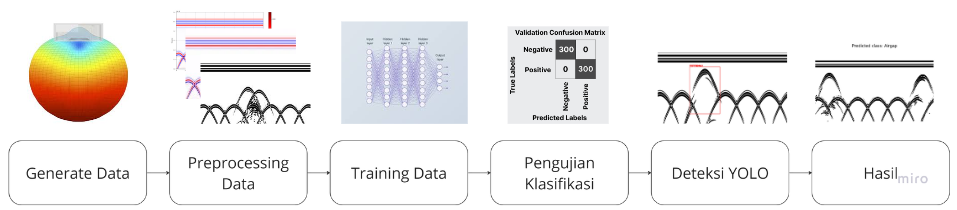
\includegraphics[scale=0.1]{gambar/bab3/flow.png}
  \caption{Blok Diagram Penelitian}
  \label{fig:metodologi}
\end{figure}

\subsection{\emph{Generate} Data}
Data sinyal GPR yang didapatkan merupakan data hasil simulasi menggunakan software gprMax. Setiap sinyal yang dihasilkan berbentuk B-Scan 2 dimensi. Pada penelitian kali ini, dihasilkan berjumlah 4000 data sinyal dengan 2000 data sinyal untuk beton berisi rongga udara dan rebar dan 2000 data sinyal untuk beton berisi rebar. 2000 File input untuk generate data sinyal berisi rongga udara dihasilkan menggunakan kode python untuk mempersingkat waktu pembuatan file input generate data. Kode python tersebut menghasilkan file input yang menghasilkan data sinyal untuk rongga udara secara acak sesuai dengan ketentuan yang telah dijabarkan pada BAB I. Data sinyal gprMax yang berisi rongga udara akan digenerate dengan menggunakan GPU secara online pada platform vast.ai karena keterbatasan hardware yang dimiliki oleh penulis. Berikut ini adalah spesifikasi dari GPU yang digunakan sebagai mana pada tabel \ref{tab:gpu}.

\begin{table}[H]
  \centering
  \begin{tabular}{|>{\bfseries}l|l|}
    \hline
    \textbf{Brand}         & NVIDIA       \\ \hline
    \textbf{Type}          & RTX 3060     \\ \hline
    \textbf{Number of GPU} & 1            \\ \hline
    \textbf{Disk Space}    & 20           \\ \hline
    \textbf{OS}            & Ubuntu 20.04 \\ \hline
    \textbf{API}           & CUDA         \\ \hline
  \end{tabular}
  \caption{spesifikasi GPU}
  \label{tab:gpu}
\end{table}

untuk data sinyal beton dengan rebar tanpa rongga udara, dihasilkan dengan cara yang sedikit berbeda. Pada awalnya, data ini digenerate dengan cara yang sama dengan data berisi rongga udara, akan tetapi setelah beberapa data, gambar sinyal yang dihasilkan memiliki banyak kemiripan. Sehingga data ini digenerate dengan cara lain. Pertama digenerate dua gambar sinyal yakni sinyal beton dengan rebar terstruktur dan gambar sinyal beton dengan rebar yang memiliki sedikit perubahan posisi, tepatnya satu rebar memiliki jarak antar rebar 10 cm. Dua gambar tersebut disatukan secara menyamping dan diproses menggunakan python untuk merubah posisi sinyal pada frame satu gambar dari dua gambar yang telah disatukan dengan perpindahan posisi sinyal secara horizontal dan vertikal per beberapa pixel. 

\subsection{\emph{Preprocessing} Data}
Sinyal gprMax yang memiliki rongga udara dalam bentuk .out yang telah digenerate, akan dilakukan proses untuk menghilangkan atribut bawaan gambar dari gprMax sehingga gambar hanya akan menampilkan gambar sinyal dan memotong ukuran gambar tersebut. Untuk gambar sinyal yang tidak memilki rongga udara, gambar tersebut akan di format ulang agar dapat diproses karena memilki format gambar yang berbeda dengan gambar hasil \emph{generaate} gprMax. Data simulasi sinyal B-Scan gprMax yang telah dipotong akan dilakukan proses binarization yang akan membuat gambar menjadi berwarna hitam putih untuk mengurangi ukuran file dari data tersebut dan model hasil training. Berikut ini adalah gambar sinyal sebelum dan sesudah diproses seperti yang dapat dilihat pada Gambar \ref{fig:beforeclean}, gambar \ref{fig:afterclean}, dan gambar \ref{fig:binary}

Berikut ini adalah contoh hasil generate data sinyal gprMax yang dapat dilihat pada Gambar \ref{fig:beforeclean} dan \ref{fig:afterclean}.

\begin{minipage}{\linewidth}
  \begin{figure} [H] \centering
    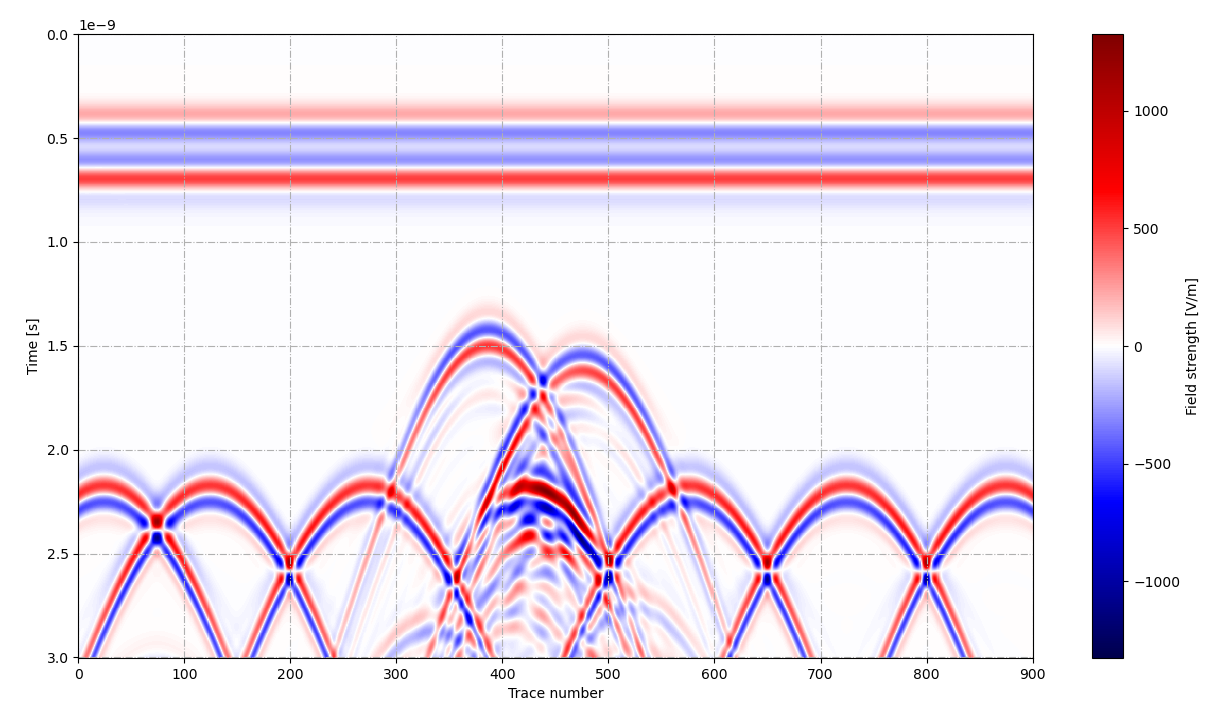
\includegraphics[scale=0.5]{gambar/bab3/beforeclean.png}
    \caption{Data Sinyal gprMax Setelah Dibersihkan}
    \label{fig:beforeclean}
  \end{figure}
\end{minipage}

\begin{minipage}{\linewidth}
  \begin{figure} [H] \centering
    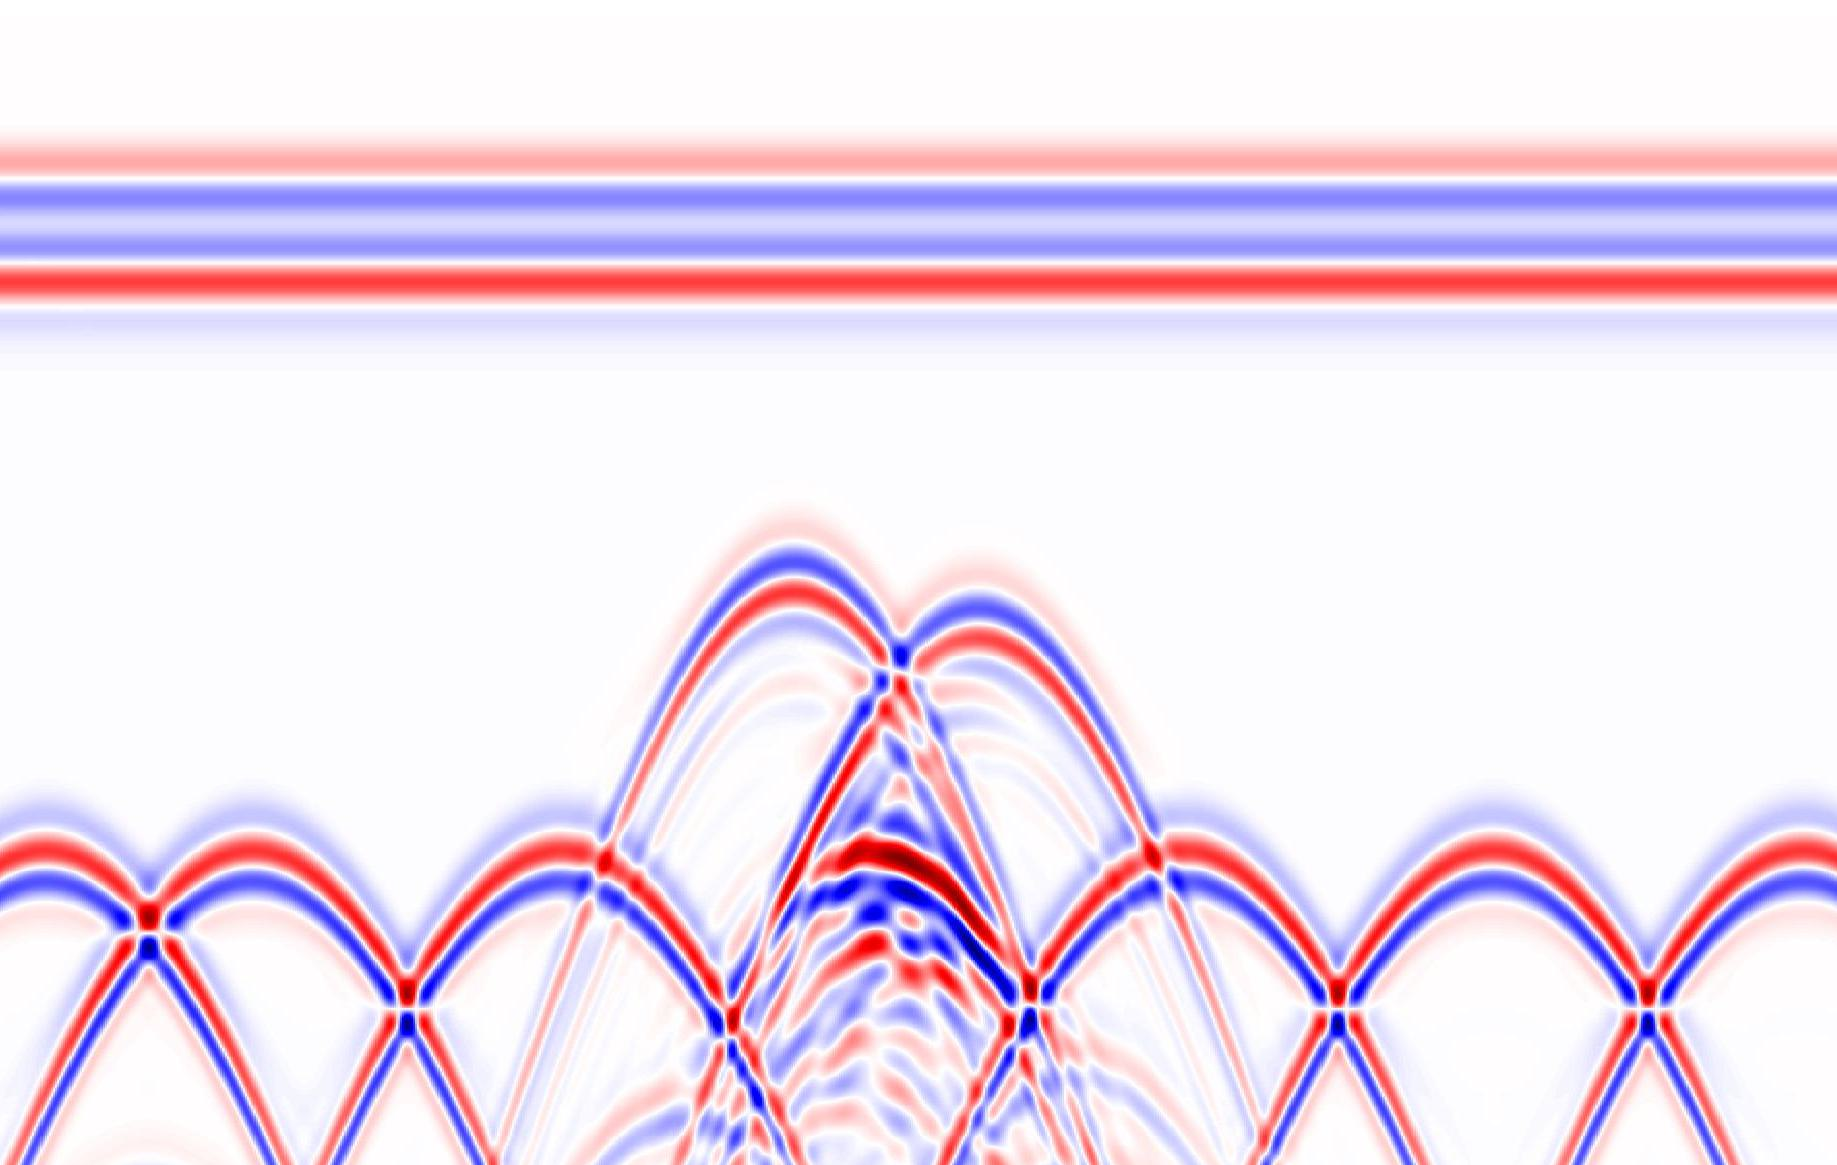
\includegraphics[scale=0.1]{gambar/bab3/afterclean.jpg}
    \caption{Data Sinyal gprMax Setelah Dibersihkan}
    \label{fig:afterclean}
  \end{figure}
\end{minipage}

\begin{figure} [H] \centering
  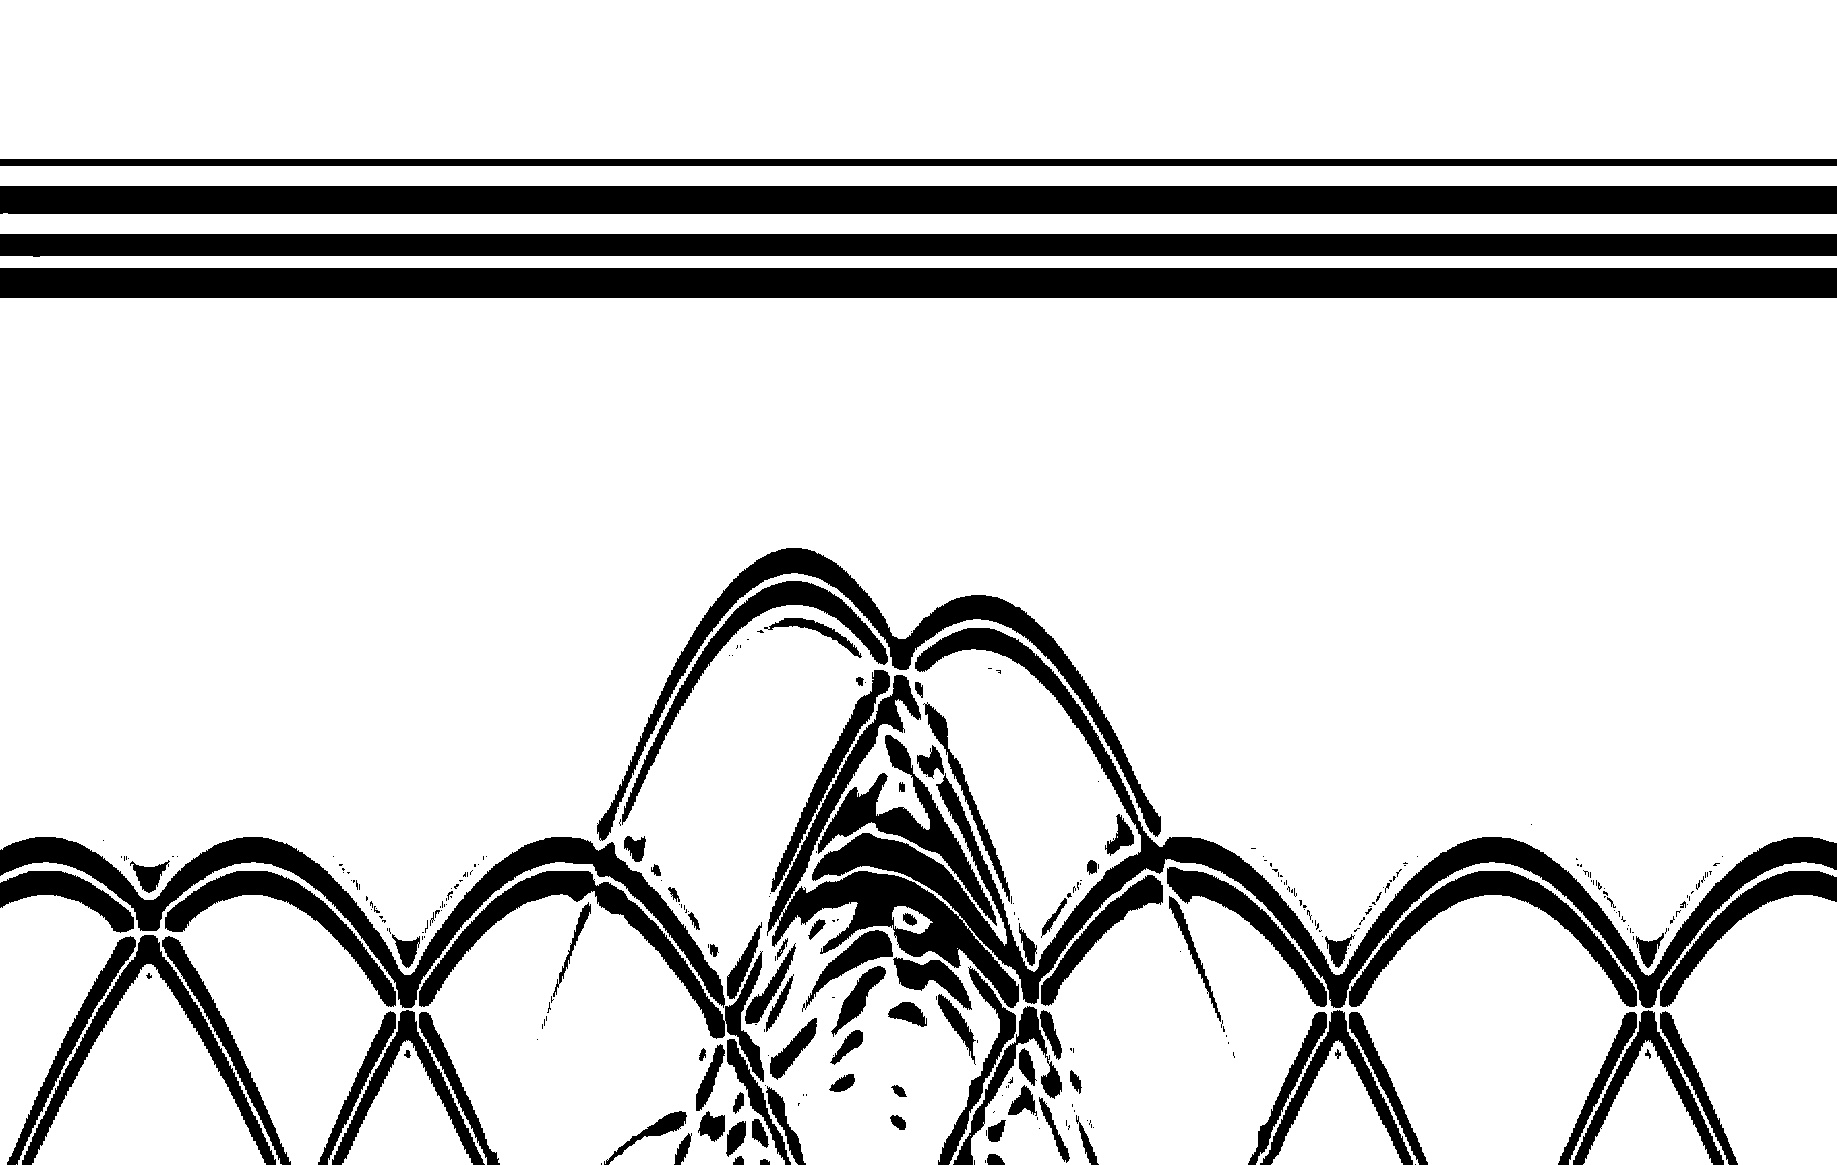
\includegraphics[scale=0.1]{gambar/bab3/binary.jpg}
  \caption{Data Sinyal gprMax Setelah Dibersihkan}
  \label{fig:binary}
\end{figure}

\subsection{\emph{Training} Data}
Dataset yang telah dihasilkan terbagi menjadi dua kelas yakni 'airgap' dan 'noarigap'. Data tersebut akan dilakukan proses training untuk klasifikasi. Terdapat dua metode klasifikasi yang digunakan yakni CNN 2-Dimensi dan Roboflow. Pada CNN 2D, diterapkan berbagai macam pembagian dataset untuk training, validasi, dan testing. Pembagian dataset yang akan diujikan untuk training, validasi, dan testing antara lain 70/20/10, 70/15/15, dan 60/20/20. Model CNN 2D yang akan digunakan untuk pembagian dataset dapat dilihat pada tabel \ref{fig:cnnarc1}.

  \begin{figure} [H] \centering
    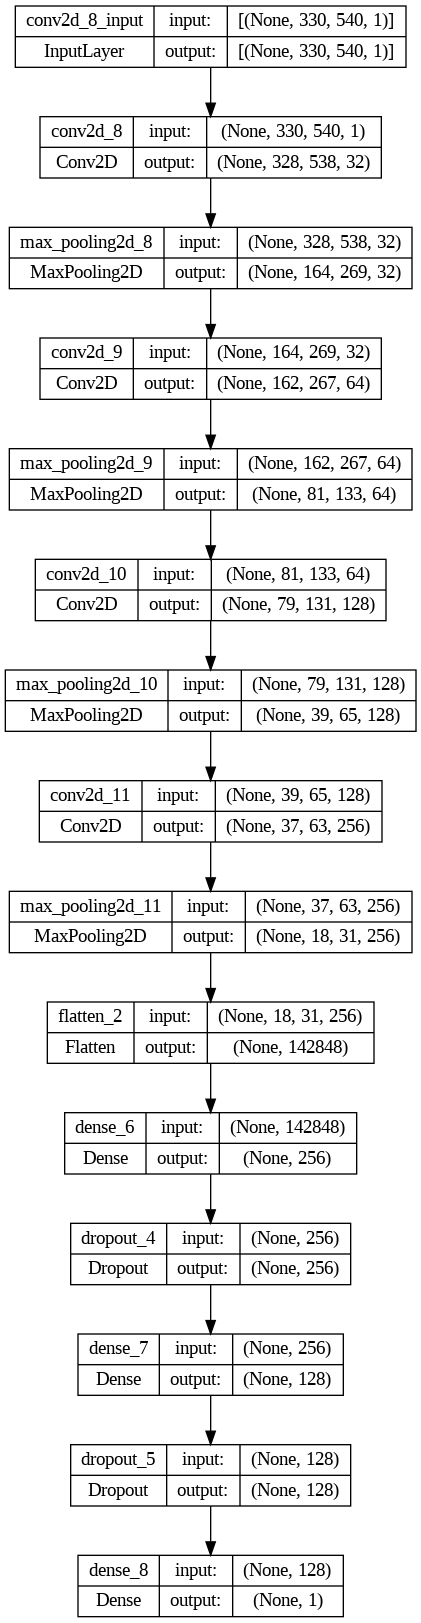
\includegraphics[scale=0.4]{gambar/bab3/cnnarc1.png}
    \caption{Arsitektur Model CNN 2D Pertama}
    \label{fig:cnnarc1}
  \end{figure}

Setelah didapatkan hasil pembagian data yang baik, pembagian data tersebut nantinya akan diterapkan pada struktur CNN 2-Dimensi yang divariasi untuk menemukan bagaimana struktur CNN 2-Dimensi yang optimal pada percobaan keempat, kelima, keenam dan ketujuh. Variasi model CNN 2D yang akan digunakan dapat dilihat pada tabel \ref{fig:cnnarc2}, tabel \ref{fig:cnnarc3}, tabel \ref{fig:cnnarc4}, dan tabel \ref{fig:cnnarc5}. CNN 2-Dimensi yang digunakan pada percobaan ini didapatkan dengan bantuan ChatGPT. Sementara itu, untuk model CNN 2D yang digunakan pada percobaan ketujuh, diambil dari peneltian yang berjudul \emph{"Classification of soil types from GPR B Scans using deep learning techniques"} \parencite{Barkataki2021}.

  \begin{figure} [H] \centering
    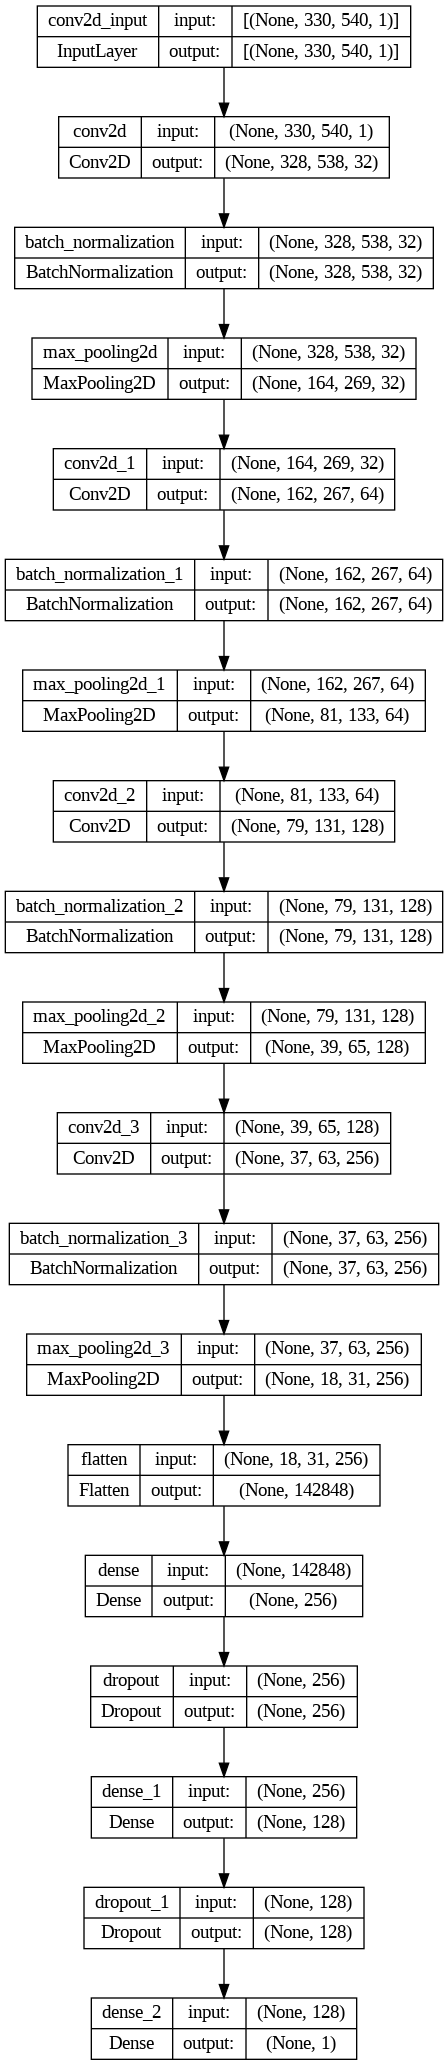
\includegraphics[scale=0.3]{gambar/bab3/cnnarc2.png}
    \caption{Arsitektur Model CNN 2D Kedua}
    \label{fig:cnnarc2}
  \end{figure}

  \begin{figure} [H] \centering
    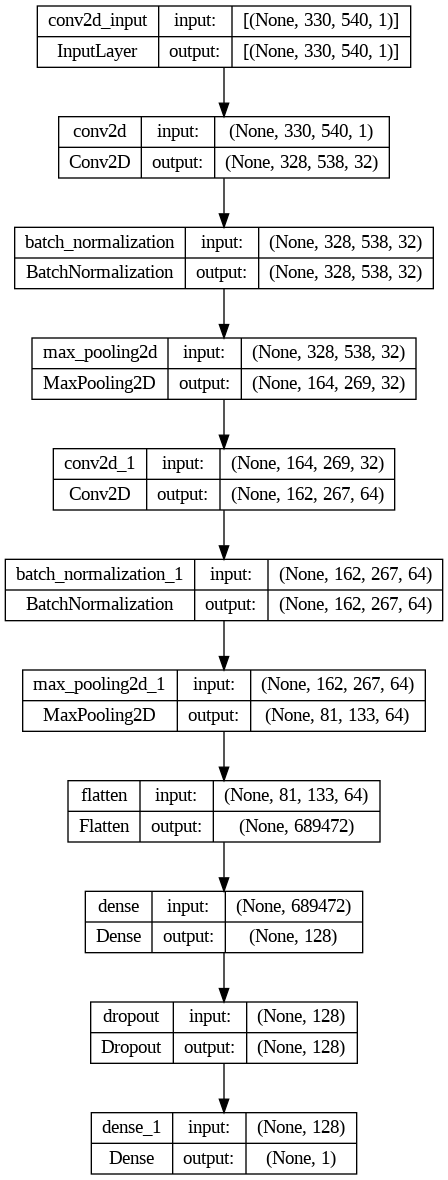
\includegraphics[scale=0.4]{gambar/bab3/cnnarc3.png}
    \caption{Arsitektur Model CNN 2D Ketiga}
    \label{fig:cnnarc3}
  \end{figure}

  \begin{figure} [H] \centering
    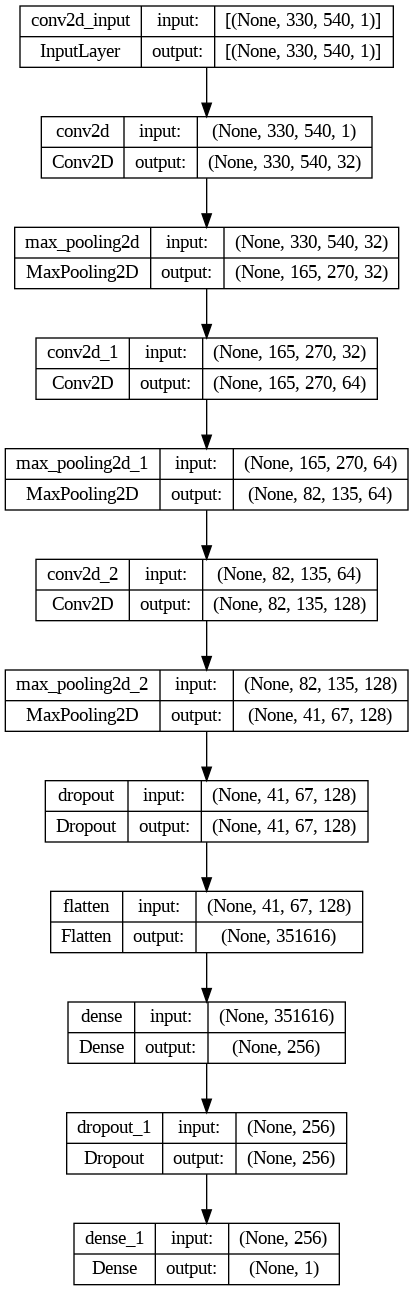
\includegraphics[scale=0.4]{gambar/bab3/cnnarc4.png}
    \caption{Arsitektur Model CNN 2D Keempat}
    \label{fig:cnnarc4}
  \end{figure}

  \begin{figure} [H] \centering
    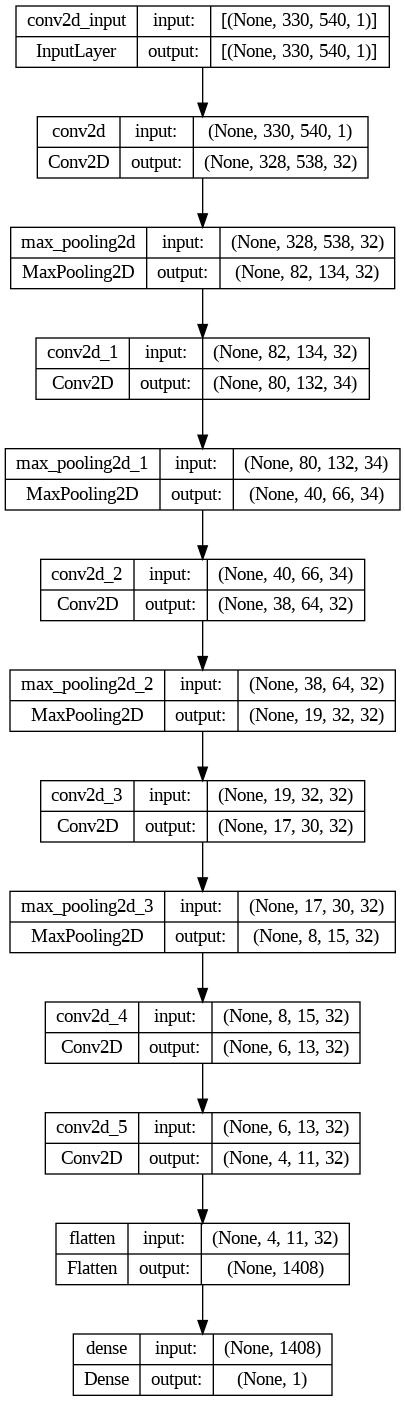
\includegraphics[scale=0.4]{gambar/bab3/cnnarc5.png}
    \caption{Arsitektur Model CNN 2D Kelima}
    \label{fig:cnnarc5}
  \end{figure}

Sementara pada Roboflow, proses klasifikasi cukup hanya dengan menetapkan gambar pada salah satu kelas. Kemudian dilakukan proses augmentasi pada data tersebut antara lain: flip (horizontal and vertical), rotate (90 degrees clockwise and counter-clockwise), crop (20\% maximum zoom), noise (up to 0.93\% pixels), dan blur (up to 1 px). Pada Roboflow, pembagian kelas awal adalah 70/20/10 untuk training, validation, dan testing. Persentase tersebut berubah setelah ditambahkan proses augmentasi menjadi 88/8/4.

\subsection{Pengujian Klasifikasi}
Pengujian klasifikasi dilakukan dengan melakukan test pada data validasi yang kemudian hasilnya akan membentuk confussion matrix. Pengujian klasifikasi juga akan dilakukan terhadap data yang dipersiapkan untuk testing diawal proses training. Pada platform, roboflow, pengujian klasifikasi cukup dilakukan dengan menguggah gambar yang hendak diuji, berikutnya platfor Roboflow akan otomatis mengklasifikasikan gambar kelas tersebut.

\subsection{Deteki YOLOv9}
YOLO yang digunakan pada training kali ini adalah YOLOv9. Versi ini dipilih karena YOLOv9 masih tergolong baru sehingga belum banyak digunakan oleh banyak orang. Model YOLOv9 ini diambil dari ultralytics berdasarkan penelitian yang berjudul \emph{"YOLOv9: Learning What You Want to Learn Using Programmable Gradient Information"} \parencite{wang2024yolov9}. Berikut ini adalah rincian dari arsitektur YOLOv9 yang digunakan pada penelitian ini:

\begin{table}[H]
  \centering
  \begin{tabular}{|c|l|c|c|c|c|c|}
    \hline
    \textbf{Index} & \textbf{Module} & \textbf{Route} & \textbf{Filters}   & \textbf{Depth} & \textbf{Size} & \textbf{Stride} \\ \hline
    0              & Conv            & -              & 64                 & -              & 3             & 2               \\ \hline
    1              & Conv            & -              & 128                & -              & 3             & 2               \\ \hline
    2              & CSP-ELAN        & 0              & 256, 128           & 2              & 1             & 1               \\ \hline
    3              & DOWN            & 1              & 256                & -              & -             & -               \\ \hline
    4              & CSP-ELAN        & 2              & 512, 256           & 2              & 1             & 1               \\ \hline
    5              & DOWN            & 4              & 512                & -              & -             & -               \\ \hline
    6              & CSP-ELAN        & 5              & 512, 512           & 2              & 1             & 1               \\ \hline
    7              & DOWN            & 6              & 512                & -              & -             & -               \\ \hline
    8              & CSP-ELAN        & 7              & 512, 512, 256      & 2              & 1             & 1               \\ \hline
    9              & SPP-ELAN        & 8              & 512, 256, 256, 512 & 3              & 1             & 1               \\ \hline
    10             & Up              & 9              & 512                & -              & -             & -               \\ \hline
    11             & Concat          & 10, 6          & 1024               & -              & -             & -               \\ \hline
    12             & CSP-ELAN        & 11             & 512, 512, 256      & 2              & 1             & 1               \\ \hline
    13             & Up              & 12             & 512                & -              & -             & -               \\ \hline
    14             & Concat          & 13, 4          & 1024               & -              & -             & -               \\ \hline
    15             & CSP-ELAN        & 14             & 256, 256, 128      & 2              & 1             & 1               \\ \hline
    16             & Down            & 15             & 256                & -              & -             & -               \\ \hline
    17             & Concat          & 16, 12         & 768                & -              & -             & -               \\ \hline
    18             & CSP-ELAN        & 17             & 512, 256, 128      & 1              & 1             & 1               \\ \hline
    19             & Down            & 18             & 512                & -              & -             & -               \\ \hline
    20             & Concat          & 19, 9          & 1024               & -              & -             & -               \\ \hline
    21             & CSP-ELAN        & 20             & 512, 512, 256      & 2              & 1             & 1               \\ \hline
    22             & Predict         & 15, 18, 21     & -                  & -              & -             & -               \\ \hline
  \end{tabular}
  \caption{Konfigurasi Jaringan YOLOv9}
  \label{tab:networkyolov9}
\end{table}

\begin{table}[H]
  \centering
  \begin{tabular}{|l|l|}
    \hline
    \textbf{Hyper Parameter}    & \textbf{Value} \\ \hline
    epochs                      & 500            \\ \hline
    optimizer                   & SGD            \\ \hline
    initial learning rate       & 0.01           \\ \hline
    finish learning rate        & 0.0001         \\ \hline
    learning rate decay         & linear         \\ \hline
    momentum                    & 0.937          \\ \hline
    weight decay                & 0.0005         \\ \hline
    warm-up epochs              & 3              \\ \hline
    warm-up momentum            & 0.8            \\ \hline
    warm-up bias learning rate  & 0.1            \\ \hline
    box loss gain               & 7.5            \\ \hline
    class loss gain             & 0.5            \\ \hline
    DFL loss gain               & 1.5            \\ \hline
    HSV saturation augmentation & 0.7            \\ \hline
    HSV value augmentation      & 0.4            \\ \hline
    scale augmentation          & 0.9            \\ \hline
    mosaic augmentation         & 1.0            \\ \hline
    MixUp augmentation          & 1.5            \\ \hline
    copy \& paste augmentation  & 0.3            \\ \hline
    close mosaic epochs         & 15             \\ \hline
  \end{tabular}
  \caption{Pengaturan Hyperparameter YOLOv9}
  \label{tab:hyperparameters}
\end{table}

\subsection{Hasil}
Hasil dari training CNN 2D nantinya akan menghasilkan grafik training, tingkat akurasi, confusion matriks, dan f1 score yang nantinya akan digunakan sebagai pertimbangan untuk mengetahui keberhasilan dari model yang telah di training. Sementara untuk hasil training dari Roboflow hanya akan menghasilkan grafik training  dan confusion matriks yang disediakan secara gratis dari platform website tersebut. Hasil training dari YOLOv9 akan menghasilkan berbagai macam metriks termasuk akurasi dan confusion matriks.

\section{Implementasi Deteksi}
\label{sec:implementasi alat}
Pada penelitian ini dikembangkan suatu website yang dapat menerima gambar sinyal GPR maupun gprMax dan melakukan klasifikasi serta deteksi rongga udara pada gambar tersebut. website ini dibangun menggunakan framework Next.js karena memiliki fungsi yang sama dengan React dan proses pemrograman yang lebih mudah. Pengguna dapat menggunakan website ini dengan mengikuti alur dari flowchart yang dapat dilihat pada gambar \ref{fig:flowuser}.

\begin{minipage}{\linewidth}
  \begin{figure} [H] \centering
    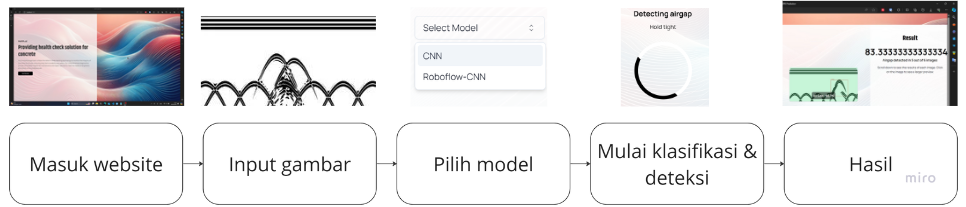
\includegraphics[scale=0.1]{gambar/bab3/flowuser.png}
    \caption{Flowchart Penggunaan Website}
    \label{fig:flowuser}
  \end{figure}
\end{minipage}

Berdasarkan flowchart diatasa, pengguna dapat mengunjungi laman website https://airgap-detect.vercel.app/ dan memasuki laman utama. Kemudian user dapat memasuki laman deteksi untuk mengunggah gambar sinyal yang ingin dideteksi keberadaan rongga udaranya. Pengguna dapat memilih model yang ingin digunakan antara model CNN 2D atau Roboflow. Setelah memilih model, pengguna dapat memulai proses klasifikasi dan deteksi. Hasil klasifikasi dan deteksi akan ditampilkan diakhir proses dengan gambar sinyal yang tidak memiliki rongga udara akan diberi filter merah dan yang memiliki rongga udara akan memilki filter hijau dengan bounding box dari YOLOv9. Hasil tersebut dapat didownload dalam bentuk zip. Website ini dideploy pada vercel dan dihosting dengan biznet. Pada pembuatan website, proses terbagi menjadi dua tahap utama yakni frontend dan backend. Berikut ini adalah flowchart tentang bagaimana website ini bekerja sebagaimana dapat dilihat pada gambar \ref{fig:webflow}.

\begin{minipage}{\linewidth}
  \begin{figure} [H] \centering
    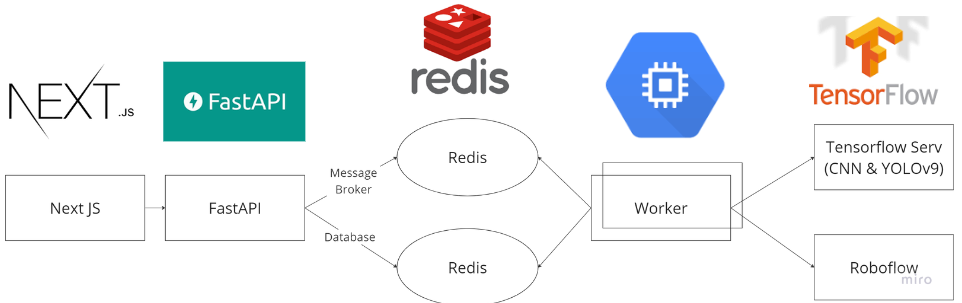
\includegraphics[scale=0.15]{gambar/bab3/webflow.png}
    \caption{Flowchart Website}
    \label{fig:webflow}
  \end{figure}
\end{minipage}

Tahap pertama yang perlu dilakukan adalah pengerjaan bagian frontend. Langkah pertama yang dilakukan adalah melakukan desain dari website tersebut. Proses desain dilakukan pada platform figma. Setelah desain selesai, langkah selanjutnya adalah melakukan implementasi desain tersebut ke dalam kode program. Proses implementasi ini dilakukan dengan menggunakan framework Next.js. Pada tahap ini, dilakukan pembuatan beberapa halaman website yang terdiri dari halaman utama, halaman upload gambar, halaman hasil klasifikasi, dan halaman hasil deteksi. Backend dibuat setelah frontend selesai dimana diperlukan pembuatan API agar frontend dapat bekerja. API yang digunakan pada pembuatan backend adalah FastAPI. FastAPI sendiri digunakan agar website dapat memproses berbagai lebih dari satu user request pada saat yang bersamaan. API ini nantinya akan terhubung dengan Redis sebagai platform database dan message broker yang mana akan menjadi perantara bagi frontend dengan virtual machine yang digunakan untuk melakukan klasifikasi dan deteksi. ketika pengguna mengunggah gambar, maka gambar akan disimpan sementara pada database Redis. Kemudian Redis akan mengirim pesan pada virtual machine sebagai worker untuk melakukan klasifikasi dan deteksi. Sebelumnya, model CNN 2-Dimensi dan YOLOv9 tidak dimasukkan ke dalam virtual machine, melainkan ke dalam Tensorflow Serving. Hal tersebut bertujuan agar model dapat diakses oleh lebih dari satu instance saat terdapat lebih dari satu request dan mengurangi jumlah memori yang akan digunakan oleh setiap instance. Model dari YOLOv9 perlu dikonversi terlebih dahulu dari pytorch ke keras (pb) agar bisa digunakan. Untuk model dari Roboflow, tidak perlu diletakkan pada Tensorflow Serving karena cukup dengan memanggil endpoint saja. Setelah model berhasil diakses, maka model akan melakukan klasifikasi dilanjut dengan deteksi YOLOv9. Hasil klasifikasi dan deteksi tersebut akan dikirimkan ke database untuk dikirimkan kembali ke user serta menghapus gambar yang telah diunggah. Berikut ini adalah contoh hasil dari website yang telah dibuat:

\begin{minipage}{\linewidth}
  \begin{figure} [H] \centering
    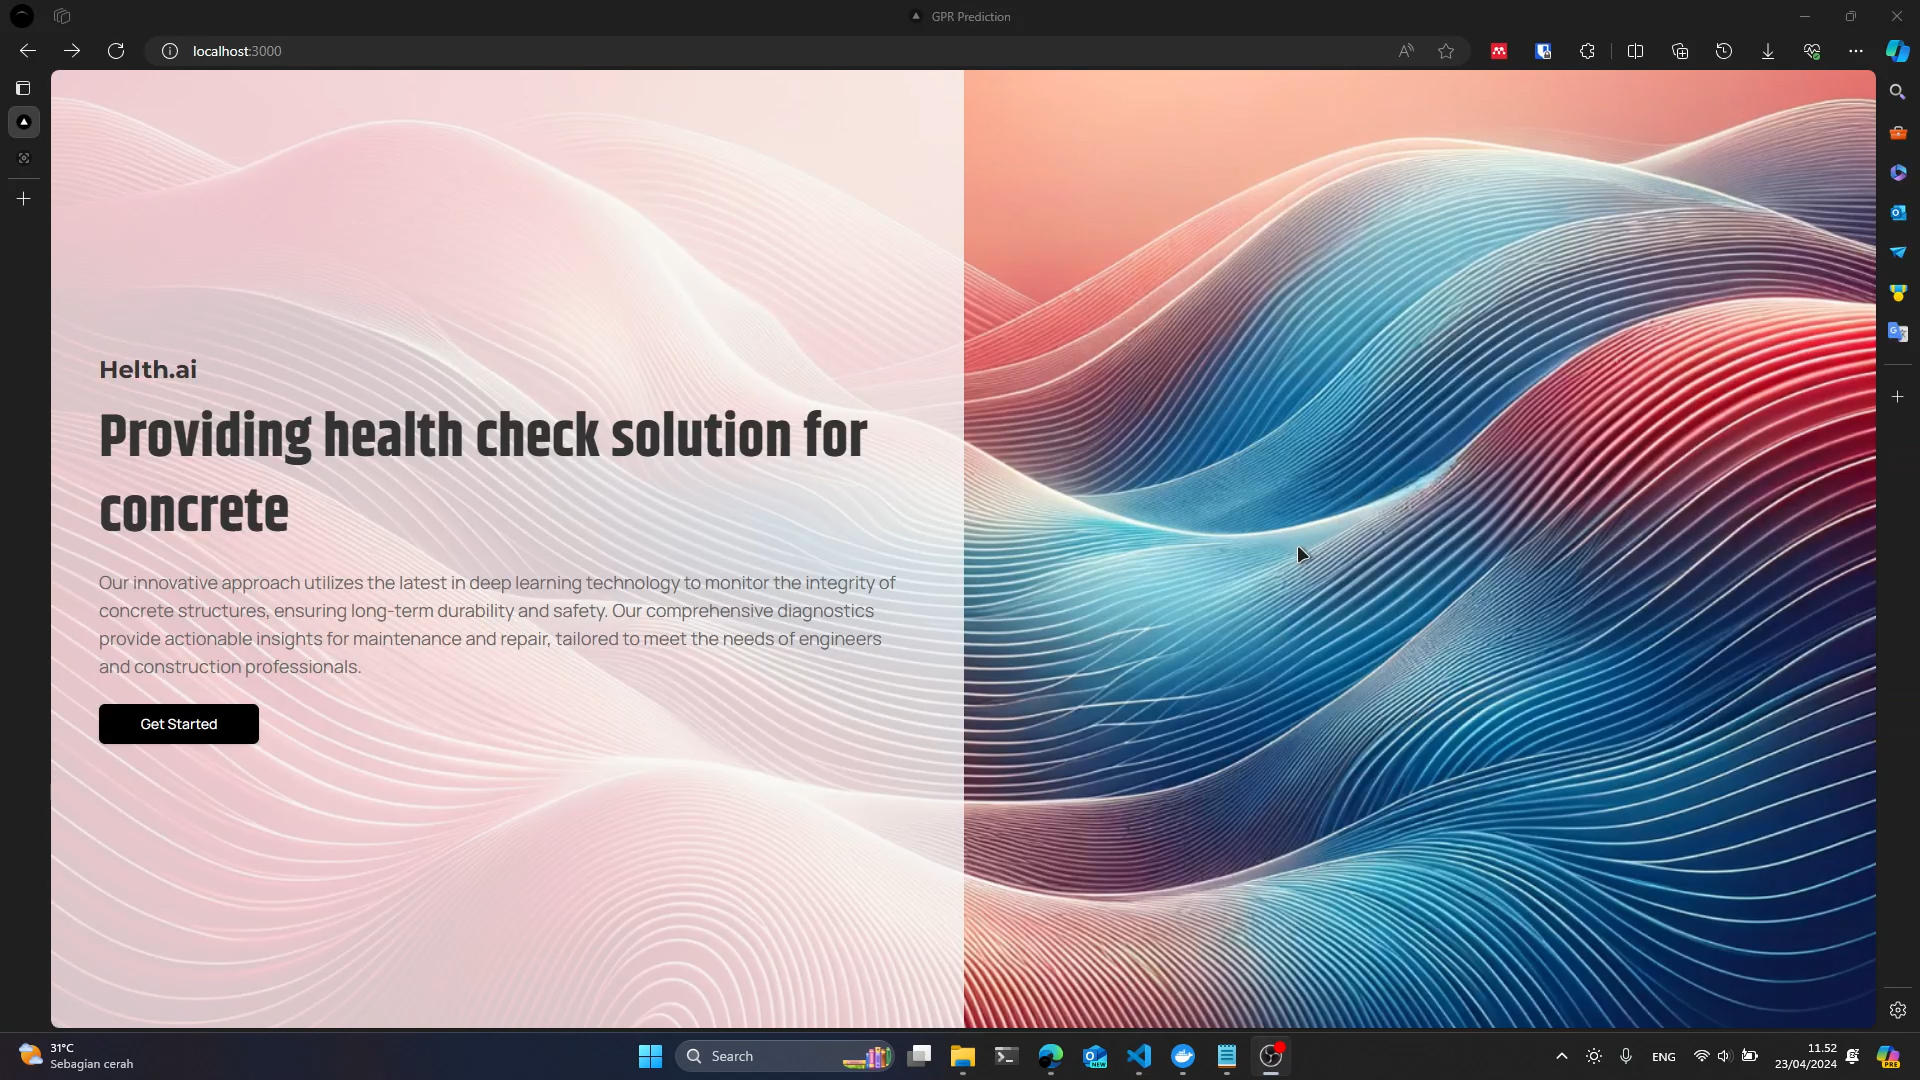
\includegraphics[scale=0.15]{gambar/bab3/web1.png}
    \caption{Gambar Platform Website 1}
  \end{figure}
\end{minipage}

\begin{minipage}{\linewidth}
  \begin{figure} [H] \centering
    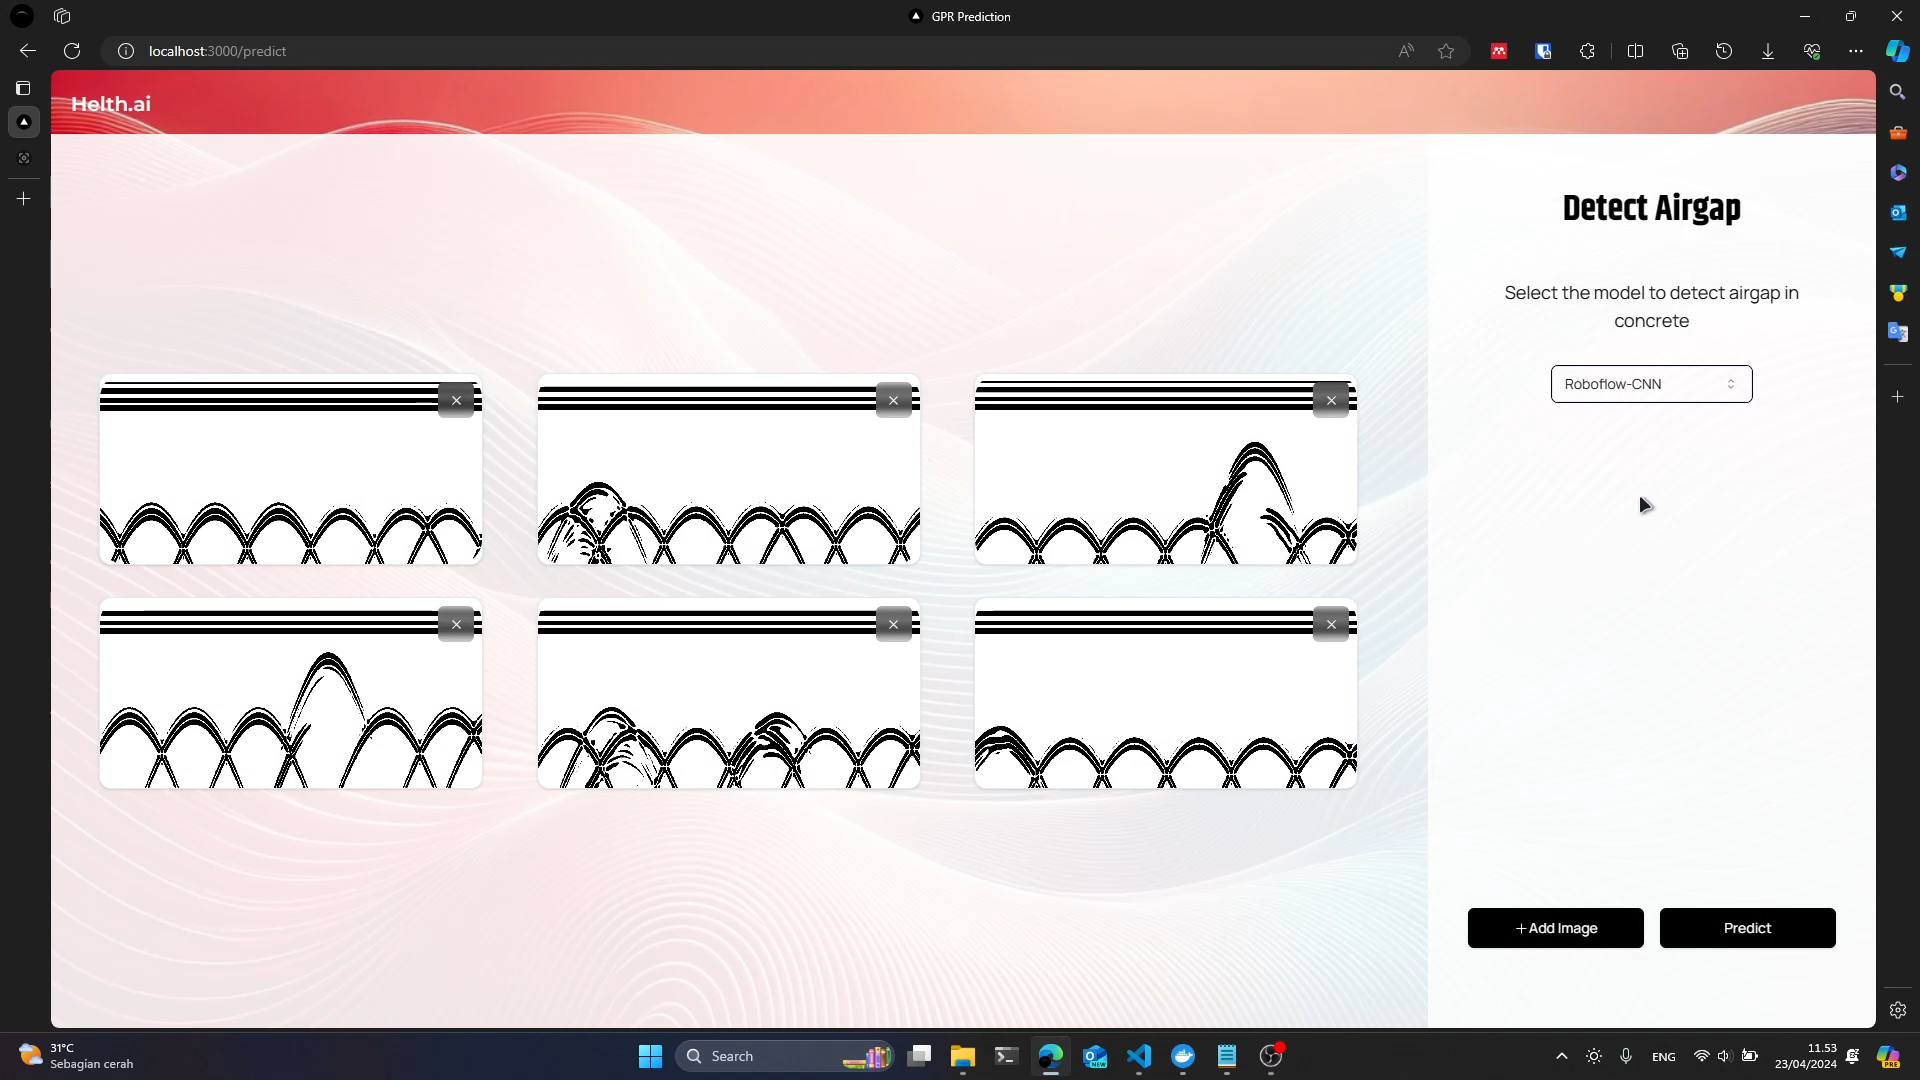
\includegraphics[scale=0.15]{gambar/bab3/web2.png}
    \caption{Gambar Platform Website 2}
  \end{figure}
\end{minipage}

\begin{minipage}{\linewidth}
  \begin{figure} [H] \centering
    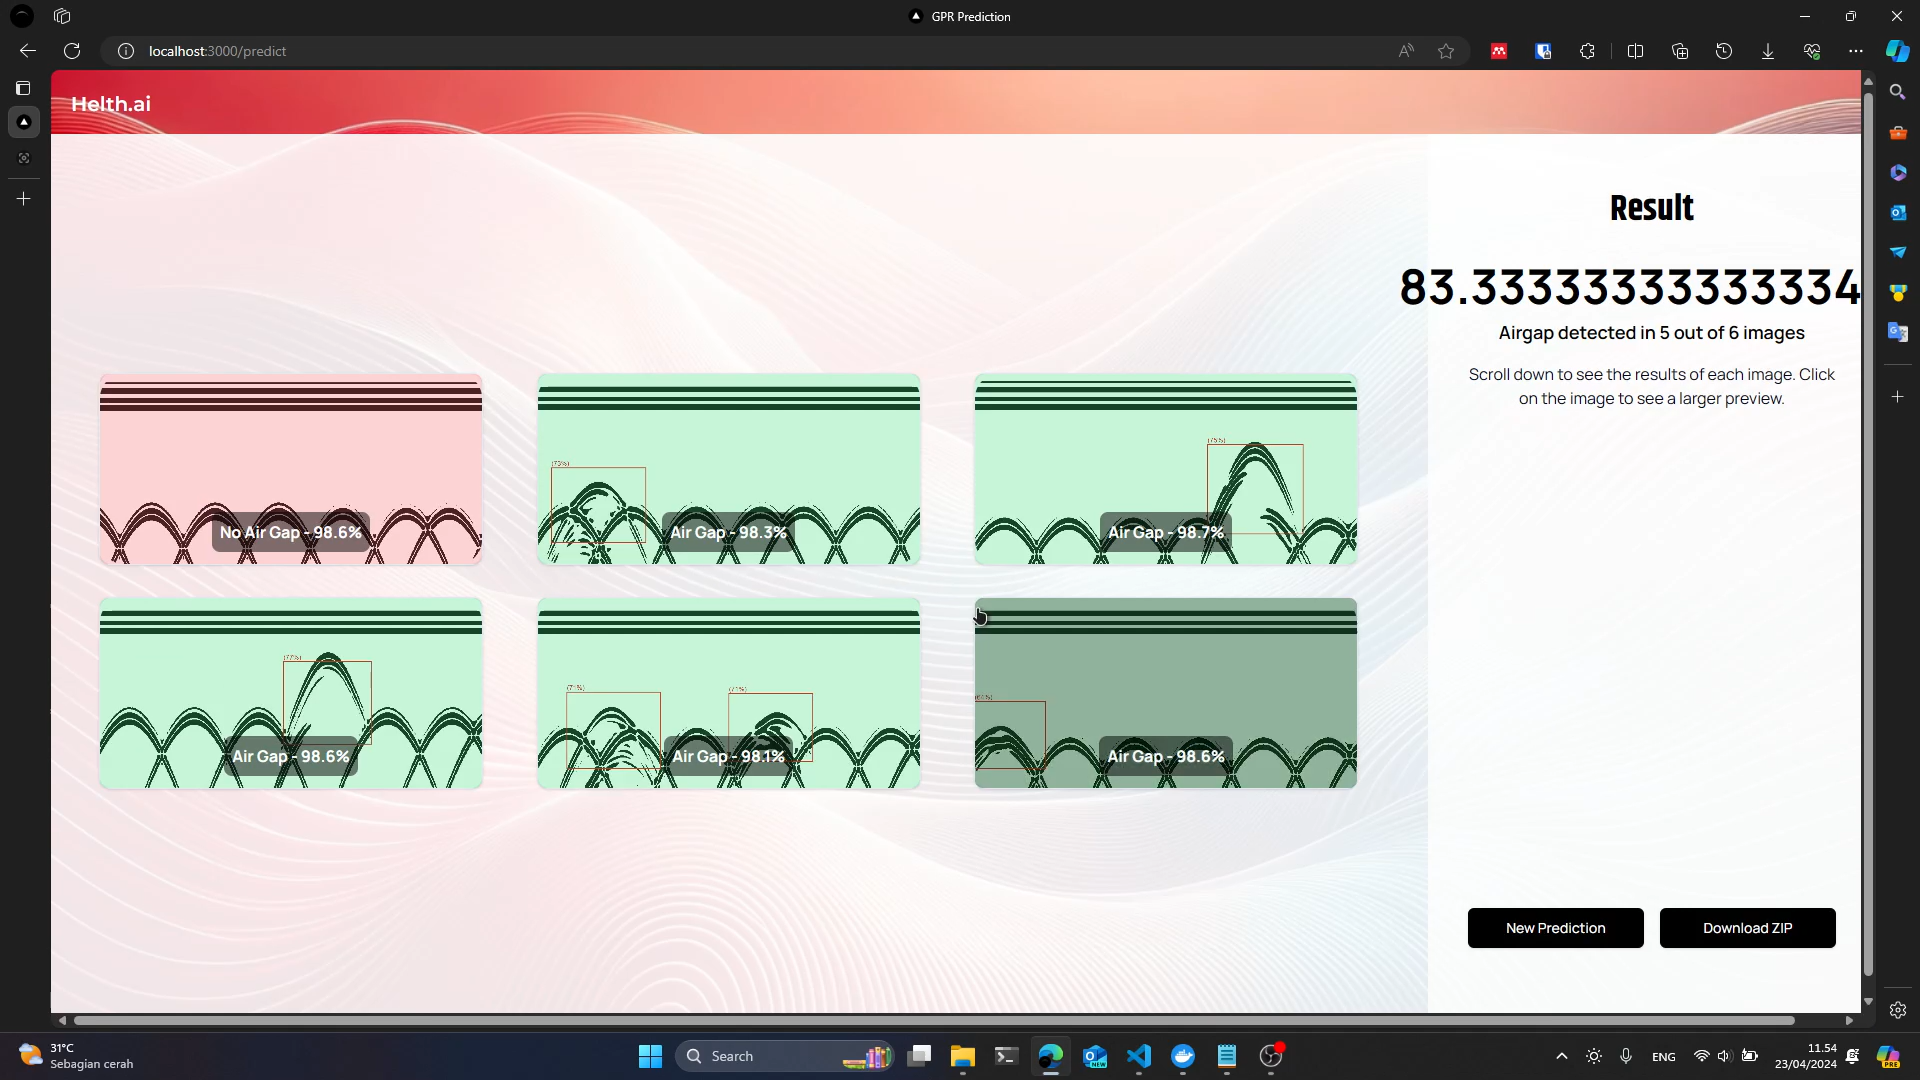
\includegraphics[scale=0.15]{gambar/bab3/web3.png}
    \caption{Gambar Platform Website 3}
  \end{figure}
\end{minipage}

\section{Kode Program}
Pada sub bab ini akan dijabarkan kode program yang digunakan pada penelitian ini.

\subsection{File Input Generate Data}
Gambar sinyal dihasilkan dengan memasukkan file input yang berisi parameter-parameter yang diperlukan untuk menghasilkan gambar sinyal. File input berisi parameter-parameter yang diperlukan untuk menghasilkan gambar sinyal. File input dihasilkan secara otomatis menggunakan python karena jumlahnya yang banyak. Berikut ini adalah flowchart dari file input generate data yang dapat dilihat pada gambar \ref{fig:generateflow}.

\begin{minipage}{\linewidth}
  \begin{figure} [H] \centering
    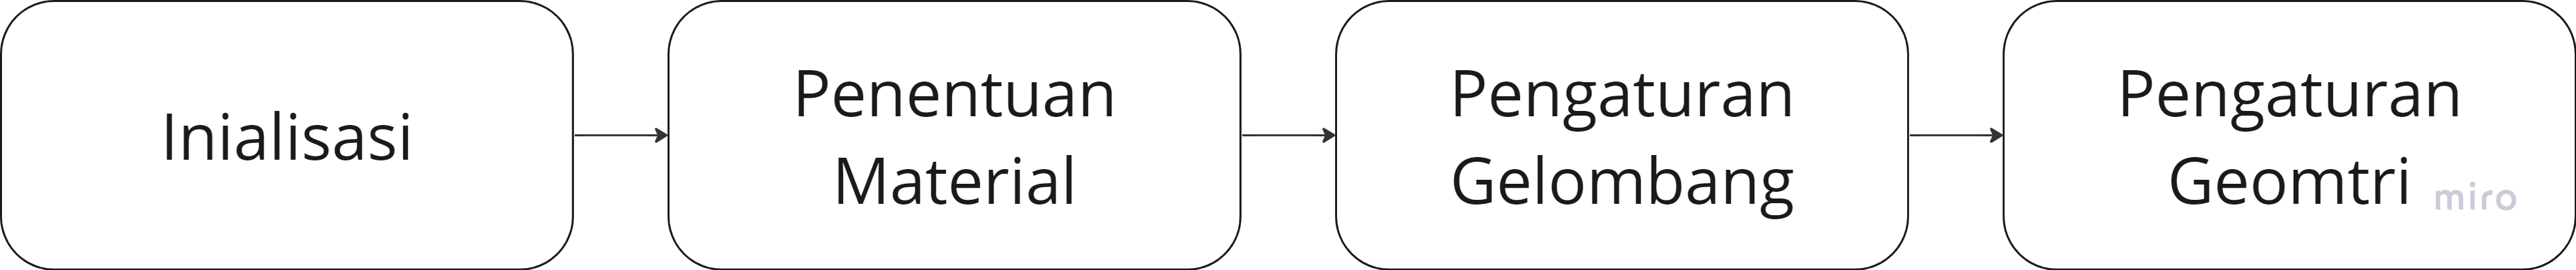
\includegraphics[scale=0.1]{gambar/bab3/generateflow.png}
    \caption{Input File Generate Data}
    \label{fig:generateflow}
  \end{figure}
\end{minipage}

\begin{algorithm}
  \caption{Simulation of B-scan from Rebar in Concrete}
  \begin{algorithmic}[1]
      \State Title: "B-scan from rebar in concrete"
      \State Define domain: 1.0 m x 0.3 m x 0.001 m
      \State Cell size: 0.001 m x 0.001 m x 0.001 m
      \State Time window: $3 \times 10^{-9}$ s
      
      \State Define material concrete: $\epsilon=7.0$, $\sigma=0.0$, $\mu=1.0$, $\chi=0.0$
      \State Define material steel: $\epsilon=12.0$, $\sigma=1.0e6$, $\mu=1.0$, $\chi=0.0$
      
      \State Create waveform: Ricker, peak frequency $4.5 \times 10^9$, name "my\_ricker"
      \State Source steps: 0.001 m x 0 m x 0 m
      \State Receiver steps: 0.001 m x 0 m x 0 m
      \State Place box: Start (0.0, 0.0, 0.0), End (1.0, 0.203, 0.001), Material concrete
      
      \State Add Hertzian dipole: Position (0.010, 0.203, 0), Waveform "my\_ricker"
      \State Place receiver: Position (0.050, 0.203, 0)
      
      \State Place cylinders: Positions and dimensions specified for steel
      \State Place cylinders: Positions and dimensions specified for free space
  \end{algorithmic}
\end{algorithm}

Pada awal program, dituliskan judul dari gelombang yang akan dihasilkan yang mana bersifat opsional. Langkah selanjutnya adalah ditentukan ukuran media yang akan dijadikan sebagai simulasi. Pada program juga diinputkan kode untuk menentukan waktu yang akan diamati pada saat berlangsungnya simulasi dan menyusun tingkat satuan terkecil untuk file input. Pada gprMax, terdapat dua material bawaan yakni udara dan \emph{pec} yang merupakan konduktor material sempurna. Pada program ini, ditentukan material yang akan digunakan pada simulasi seperti rebar dan beton yang mana parameternya diambil berdasarkan penelitian terdahulu yang menggunakan gprMax.

Langkah selanjutnya diatur tipe gelombang yakni Ricker wavelet yang mana merupakan gelombang yang paling sering digunakan pada simulasi GPR. Diatur pula letak \emph{transmitter} dan \emph{receiver} yang akan digunakan pada simulasi yang ketinggiannya sama dengan ketinggian/ketebalan dari beton yang akan dibuat. Pergerakan dari \emph{transmitter} dan \emph{receiver} diatur untuk mampu berpindah posisi hingga sekecil 1 mm per langkah. Hal ini dilakukan untuk mendapatkan data sinyal yang lebih banyak dan akurat. Terakhir, ditentukan objek yang nantinya akan ada didalam simulasi seperti beton, rebar, dan rongga udara yang mana masing-masing objek memiliki parameter tersendiri. Pada program ini, beton menggunakan parameter \#box karena medianya kotak, rebar menggunakan parameter \#cylinder karena medianya silinder, dan rongga udara menggunakan parameter \#cylinder rongga udara memiliki bentuk yang abstrak.

\subsection{Generate File Input gprMax dengan Rongga Udara}
Program ini dirancang untuk melakukan proses generate file input gprMax dengan rongga udara. Hal tersebut dilakukan karena proses pembuatan file input gprMax dengan rongga udara dalam jumlah besar membutuhkan waktu yang lama. Program ini dibuat dengan menggunakan Python, berikut ini adalah flowchart tentang bagaimana program ini bekerja sebagaimana dapat dilihat pada gambar \ref{fig:flowgpu}.

\begin{figure} [H] \centering
  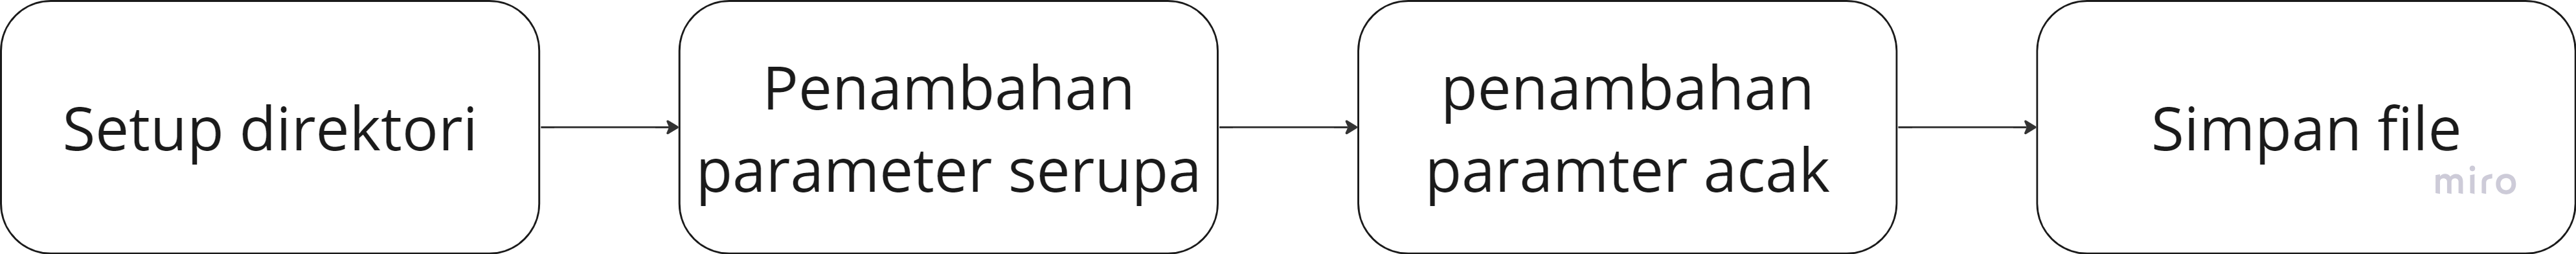
\includegraphics[scale=0.1]{gambar/bab3/flowmakein.png}
  \caption{Flowchart Setup GPU}
  \label{fig:flowmakein}
\end{figure}

\begin{algorithm}
  \caption{Generate gprMax Simulation Files}
  \begin{algorithmic}[1]
  \Function{GenerateAirgapCylinders}{$file, boxHeight$}
      \State $xMin, xMax \gets 0.05, 0.95$
      \State $yMin, yMax \gets 0.090, boxHeight - 0.05$
      \State $airgapCount \gets$ Random integer from 1 to 2
      \For{$i \gets 1$ \textbf{to} $airgapCount$}
          \State $cylinderCount \gets$ Random integer from 3 to 5
          \State $xPosition \gets$ Random float between $xMin$ and $xMax$
          \State $yPosition \gets$ Random float between $yMin$ and $yMax$
          \For{$j \gets 1$ \textbf{to} $cylinderCount$}
              \State $radius \gets$ Random float from 0.005 to 0.0175
              \State Write cylinder data to $file$
              \State Adjust $xPosition$ and $yPosition$ within bounds
          \EndFor
      \EndFor
  \EndFunction
  \State
  \Function{GenerateGprMaxFiles}{}
      \State Create directory "airgap"
      \State $totalFiles \gets 2000$
      \For{$fileNumber \gets 1$ \textbf{to} $totalFiles$}
          \State $boxHeight \gets$ Random float between 0.190 and 0.210
          \State Create file with initial configuration
          \State Write steel cylinder configuration to file
          \State \Call{GenerateAirgapCylinders}{$file, boxHeight$}
          \State Print file creation message
      \EndFor
  \EndFunction
  \end{algorithmic}
  \end{algorithm}

Pada langkah awal, dilakukan inisialisasi dengan membuat folder baru sebagai tempat disiapkannya hasil generate file input gprMax. Kemudian, dilakukan perulangan untuk membuat file text yang berisi struktur dari sinyal yang akan digenerate. Program akan menambahkan parameter-parameter yang akan dimiliki oleh semua file input (parameter serupa) terlebih dahulu di awal seperti judul file, ukuran domain, rentang waktu, tingkat kerincian, mterial, jenis gelombang, dan pergerakan dari transmitter dan receiver gelombang. Setelah itu, dilakukan penambahan baris kode dengan parameter yang sifatnya akan divariasi secara acak. Parameter awal adalah dimensi beton yang berukuran panjang 1 meter variasi ketebalan antara 19 cm hingga 21 cm. Ketebalan dari beton ini akan menentukan posisi ketinggian dari transmitter dan receiver yang akan ditambahkan setelahnya. Selanjutnya, akan ditambahkan parameter rebar yang memiliki material besi dengan diameter 14 mm dengan setiap rebar akan memiliki ketinggian yang sama. Ketinggian dan posisi secara horizontal ini akan berubah setiap filenya dengan rebar memiliki variasi ketinggian antara 9 cm hingga 11 cm sementara posisi horizontal rebar akan bertambah sebanyak 1 mm setiap filenya yang mana apabila posisi rebar secara horizontal melebihi panjang rebar, maka kelebihan posisi tersebut akan ditempatkan pada awal posisi beton secara horizontal. Terkahir adalah parameter rongga udara yang akan ditempatkan secara acak pada beton. Rongga udara udara bisa terdiri dari satu atau lebih silinder dengan diameter antara 2 cm hingga 7 cm yang letak ketinggiannya akan berada diantara 5 cm hingga titik tertinggi beton dikurangi 5 cm. Posisi rongga udara secara horizontal akan diletakkan secara acak. Setelah semua parameter ditambahkan, file akan disimpan dalam format .in.

\subsection{Setup GPU untuk Generate Data}
Dalam, penggunaan GPU untuk mempercepat proses generate data, diperlukan pengaturan GPU terlebih dahulu agar GPU dapat digunakan. Berikut ini adalah flowchart dari setup GPU untuk generate data yang dapat dilihat pada gambar \ref{fig:flowgpu}.

\begin{figure} [H] \centering
  
\includegraphics[scale=0.1]{gambar/bab3/flowgpu.png}
  \caption{Flowchart Setup GPU}
  \label{fig:flowgpu}
\end{figure}

\begin{algorithm}
\caption{Setup Miniconda and Configure gprMax Environment}
\begin{algorithmic}[1]
\State Echo "Creating Miniconda directory..."
\State Execute "mkdir -p \textasciitilde/miniconda3"
\State Echo "Downloading Miniconda installer..."
\State Execute "wget https://repo.anaconda.com/miniconda/Miniconda3-latest-Linux-x86\_64.sh -O \textasciitilde/miniconda3/miniconda.sh"
\State Echo "Installing Miniconda..."
\State Execute "bash \textasciitilde/miniconda3/miniconda.sh -b -u -p \textasciitilde/miniconda3"
\State Echo "Removing Miniconda installer..."
\State Execute "rm -rf \textasciitilde/miniconda3/miniconda.sh"
\State Echo "Initializing Conda for bash..."
\State Execute "\textasciitilde/miniconda3/bin/conda init bash"
\State Execute "source ./\.bashrc"
\State Echo "Updating Conda..."
\State Execute "conda update conda -y"
\State Echo "Installing Git..."
\State Execute "conda install git -y"
\State Echo "Cloning gprMax repository..."
\State Execute "git clone https://github.com/MaulanaGilang/gprMax.git"
\State Echo "Changing directory to gprMax..."
\State Execute "cd gprMax"
\State Echo "Creating Conda environment from file..."
\State Execute "conda env create -f conda\_env.yml"
\State Echo "Activating gprMax environment..."
\State Execute "conda activate gprMax"
\State Echo "Building gprMax..."
\State Execute "python setup.py build"
\State Echo "Installing gprMax..."
\State Execute "python setup.py install"
\State Echo "Installing PyCUDA..."
\State Execute "pip install pycuda
\State Echo "Setup complete. gprMax is ready to use."
\end{algorithmic}
\end{algorithm}

Pada awal pengaturan GPU, GPU diakses melalui ssh yang terhubung dengan ssh key milik PC penulis. Setelah terhubung, dibuat folder baru untuk instalasi miniconda. Instalasi miniconda dilakukan dengan melakukan replikasi repositori github dan menjalankan file bash yang ada pada repositori tersebut. Setelah instalasi selesai, dilakukan pembaruan terhadap versi conda dan intalasi Git untuk proses instalasi gprMax. Proses instalasi gprMax dilakukan dengan melakukan replikasi repositori Github. Sebelum, menjalankan instalasi, dibuat environment baru untuk gprMax dan mengaktifkannya. Setelah aktif, dijalankan kode python dari repositori tersebut untuk melakukan setup gprMax. Langkah terakhir adalah melakukan instalasi PyCUDA agar proses generate data dapat menggunakan GPU.

\subsection{Generate Data Sinyal GPR}
Program ini dirancang untuk melakukan proses generate sinyal hasil simulasi file input untuk gprMax. Program ini dibuat dengan menggunakan python dan menggunakan library gprMax untuk menghasilkan data sinyal. Program ini akan menghasilkan data sinyal berupa gambar B-Scan 2 dimensi yang kemudian akan dijadikan sebagai data training untuk klasifikasi. Berikut ini adalah flowchart dari generate data yang dapat dilihat pada gambar \ref{fig:autoflow} dan \ref{fig:generatefloor}.

\begin{minipage}{\linewidth}
  \begin{figure} [H] \centering
    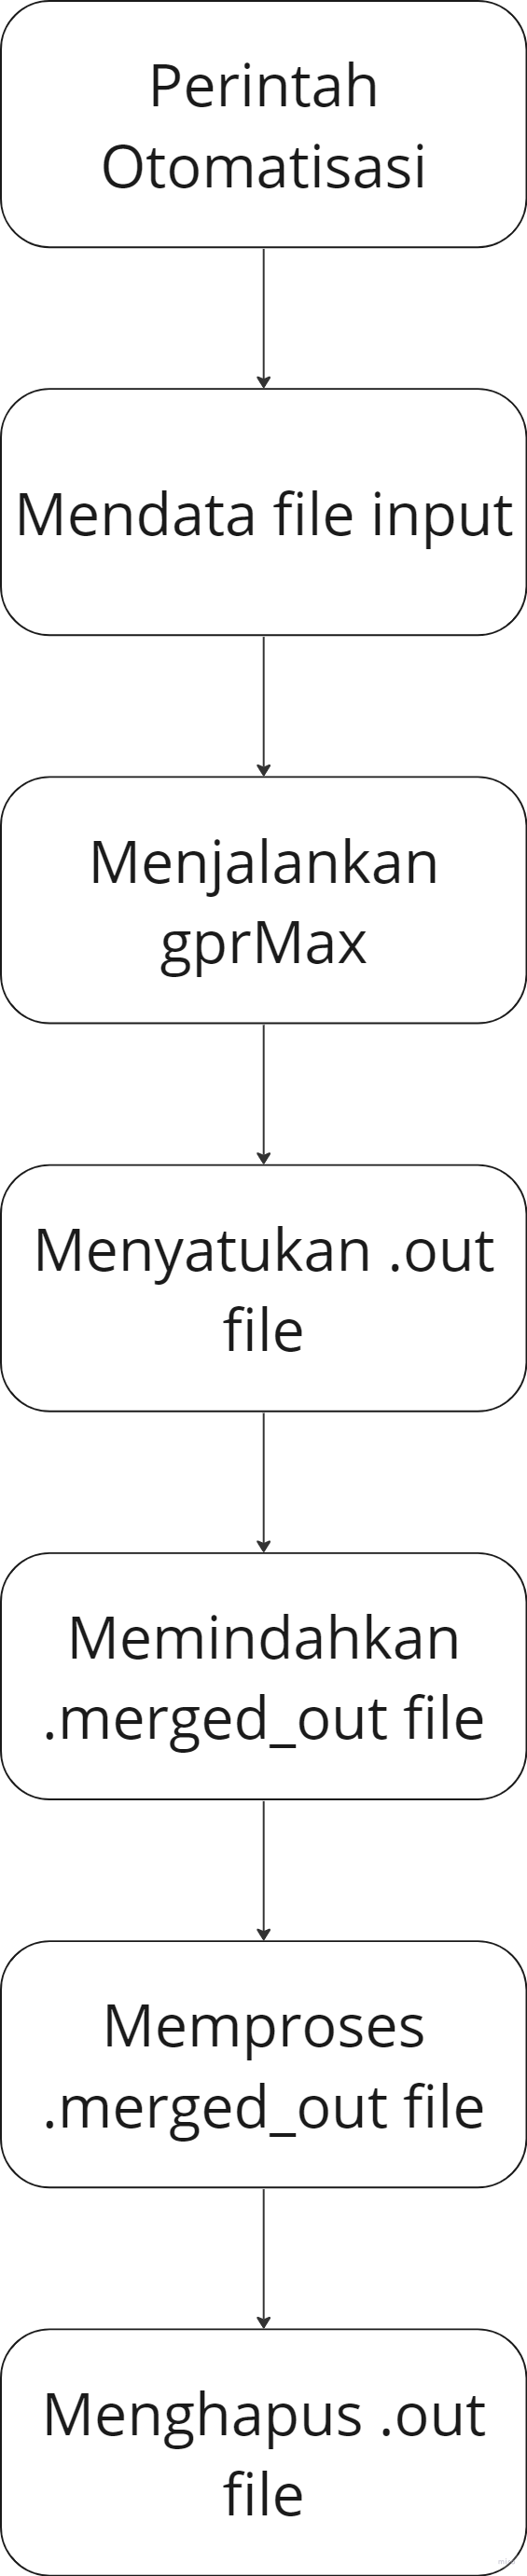
\includegraphics[scale=0.1]{gambar/bab3/autoflow.png}
    \caption{Kode Otomatiasi Generate Data}
    \label{fig:autoflow}
  \end{figure}
\end{minipage}

\begin{algorithm}
  \caption{Process GPRMax Output Files}
  \begin{algorithmic}[1]
  \Function{NaturalKeys}{text}
      \State Parse text and return parts as integers if they are digits or as text otherwise.
  \EndFunction
  \State
  \Function{ListInFilesRecursive}{directory}
      \State Recursively list all .in files in the directory.
      \State Return a dictionary of filenames without extension as keys and paths as values.
  \EndFunction
  \State
  \Function{RunGprMax}{file\_path, n, use\_gpu}
      \State Construct and run a command to execute gprMax with optional GPU usage.
  \EndFunction
  \State
  \Function{MergeOutputFiles}{directory, file\_without\_ext}
      \State Merge output files based on the .in filename and delete the original .out files.
  \EndFunction
  \State
  \Function{EnsureDirectoryExists}{directory}
      \State Create the directory if it does not exist.
  \EndFunction
  \State
  \Function{MoveOutputFile}{source\_path, dest\_directory}
      \State Move the output file to a specified directory, ensuring the directory exists.
      \State Return the new path.
  \EndFunction
  \State
  \Function{ProcessFile}{file\_path, rxnumber, rxcomponent, non\_greyscale\_dir, greyscale\_dir}
      \State Generate and save color and cropped grayscale images from the output data of gprMax.
  \EndFunction
  \State
  \Procedure{Main}{args}
      \State Parse input directory, indices and settings from command-line arguments.
      \State Initialize directories and prepare file processing.
      \For{each file to process within index range}
          \State Run gprMax simulation.
          \If{merge is enabled}
              \State Merge output files.
              \State Move and process merged file.
          \EndIf
          \State Increment processed files count.
      \EndFor
      \State Clean up any remaining processed files.
  \EndProcedure
  \end{algorithmic}
  \end{algorithm}

Pada program ini, pertama-tama dilakukan import library yang dibutuhkan. Selanjutnya, dilakukan pembacaan file input yang telah dibuat sebelumnya. File input tersebut berisi parameter-parameter yang diperlukan untuk menghasilkan gambar sinyal. Setelah itu, program akan melakukan iterasi sebanyak jumlah data yang diinginkan. Pada setiap iterasi, program akan menghasilkan gambar sinyal berdasarkan parameter yang ada pada file input dengan menjalankan software gprMax. Saat setelah selesai generate, setiap file input akan menghasilkan file output berupa potongan-potongan sinyal dengan format .out yang akan disatukan menjadi satu file dengan format .merged.out File ini kemudian akan dipindahkan ke folder yang telah disediakan dan akan menghapus semua file awal berformat .out untuk mengurangi memori yang digunakan oleh GPU. File yang dipindahkan tersebut akan dibaca dan diubah menjadi gambar sinyal menggunakan python. Gambar sinyal yang telah dihasilkan kemudian akan diproses agar parameter bawaan gambar dari gprMax hilang dan hanya menampilkan gambar sinyal saja serta memotong ukuran gambar tersebut.

\begin{minipage}{\linewidth}
  \begin{figure} [H] \centering
    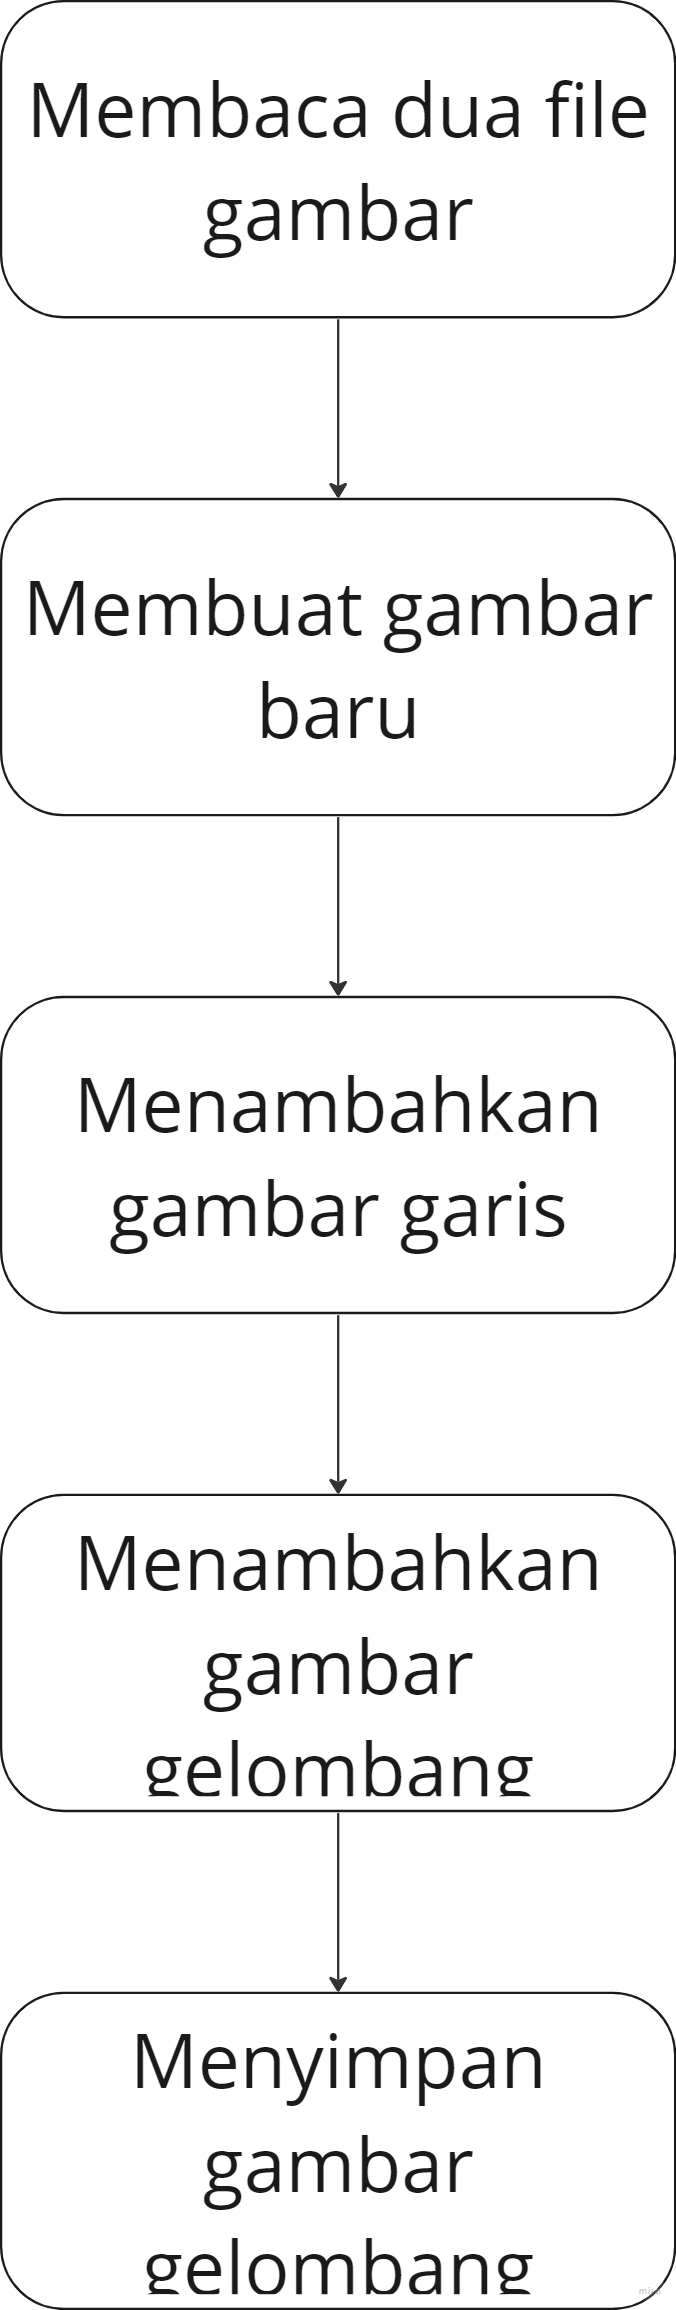
\includegraphics[scale=0.1]{gambar/bab3/generatefloor.png}
    \caption{Input File Generate Data}
    \label{fig:generatefloor}
  \end{figure}
\end{minipage}

\begin{algorithm}
  \caption{Image Manipulation and Transformation}
  \begin{algorithmic}[1]
  \State Load line and wave images from 'noairgap' directory.
  \State Create a new transparent RGBA image 'result\_img' with dimensions 1860x1160.
  \State Paste the line image onto 'result\_img' at position (0,0).
  
  \Function{TransformAndSave}{wave\_img, result\_img, shift\_x, shift\_y, crop\_size, file\_name}
      \State Create a copy of 'result\_img' to 'temp\_img'.
      \State Paste 'wave\_img' onto 'temp\_img' with specified shifts 'shift\_x' and 'shift\_y'.
      \State Repaste the line image onto 'temp\_img' at position (0,0).
      \State Crop 'temp\_img' according to 'crop\_size'.
      \State Save the cropped image to 'file\_name'.
  \EndFunction
  
  \State Calculate number of images to be generated.
  \State Initialize a counter to zero.
  \For{each horizontal shift from -wave width + 1860 to 0 step by 5}
      \For{each vertical shift from 0 to 100 step by 20}
          \State Construct file name for output image.
          \State \Call{TransformAndSave}{wave\_img, result\_img, horizontal shift, vertical shift, crop size, file name}
          \State Increment counter by one.
      \EndFor
  \EndFor
  
  \end{algorithmic}
  \end{algorithm}

Untuk program generate data sinyal gprMax yang tidak memiliki rongga udara, data ini dihasilkan dengan cara yang berbeda karena tidak banyak perbedaan pada setiap gambar sinyal yang dihasilkan. Untuk menjalan program ini, dibutuhkan gambar sinyal tanpa rongga udara hasil generate gprMax dengan gambar pertama adalah gambar normal dan gambar kedua adalah gambar sinyal dengan rebar yang memiliki sebuah rebar yang tidak berjarak 15 cm. Selanjutnya, kedua gambar tersebut disatukan secara horizontal dan dipotong bagian sinyalnya. Selanjutnya, diambil gambar garis pada salah satu gambar dengan cara dipotong. Dua gambar tersebut nantinya akan menjadi file input untuk augmentasi tersebut. Pada program, akan dibuat sebuah gambar baru dengan ukuran 1860x1160 piksel dengan latar belakang yang transparan. Kemudian, akan ditambahkan gambar garis pada bagian atas gambar tersebut. Selanjutnya ditambahkan gambar sinyal dibagian bawah gambar garis dengan ketentuan setiap gambar sinyal tersebut akan dipindahkan posisinya per gambar secara horizontal sebanyak 5 piksel hingga menyentuh batas gambar sinyal secara horizontal dan secara vertikal ke bawah 100 piksel dengan perpindahan 20 piksel per gambar. Gambar sinyal dan garis akan menimpa gambar latar belakang sehingga tercipta gambar sinyal baru. Gambar sinyal yang telah dihasilkan nantinya akan disimpan pada folder yang telah disediakan.

\subsection{\emph{Preprocessing} Data}
Program berikut ini bertujuan untuk melakukan \emph{preprocessing} data sinyal yang telah dihasilkan dari proses generate data. Program ini dibuat menggunakan python. Berikut ini adalah flowchart dari \emph{preprocessing} data yang dapat dilihat pada gambar \ref{fig:preflow1} dan \ref{fig:preflow2}

\begin{figure} [H] \centering
  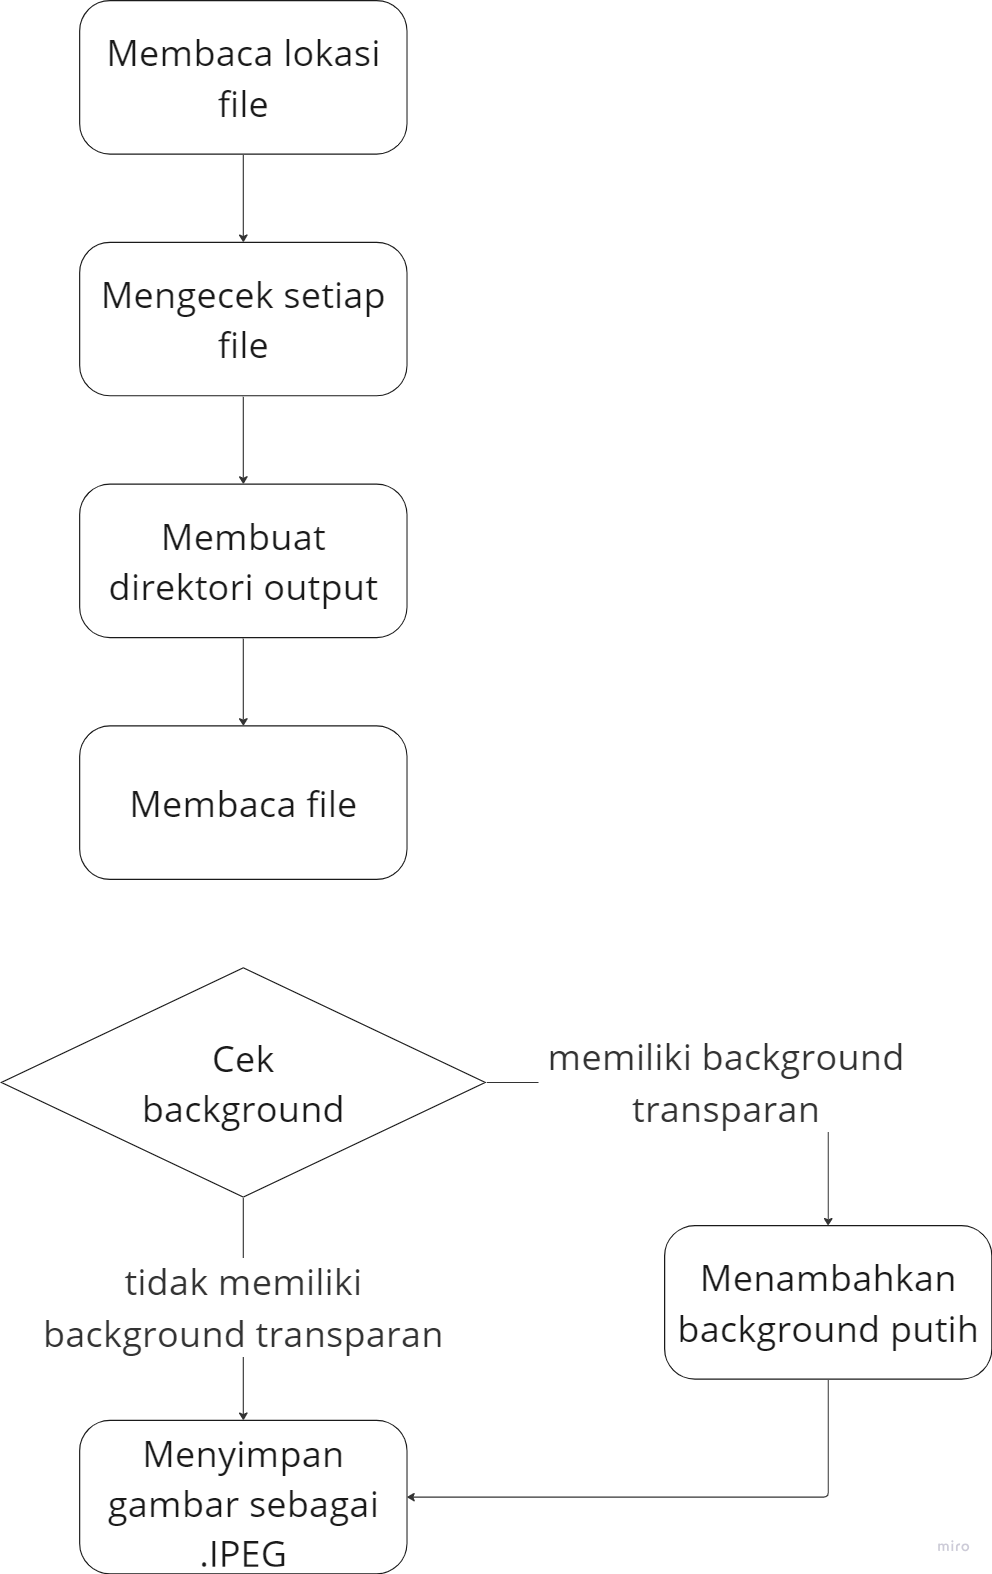
\includegraphics[scale=0.1]{gambar/bab3/preflow1.png}
  \caption{Mengubah Format Gambar Sinyal}
  \label{fig:preflow1}
\end{figure}

\begin{algorithm}
  \caption{Convert Directory Images to JPEG Format}
  \begin{algorithmic}[1]
  \Procedure{ConvertDirectoryToJPEG}{input\_dir, output\_base\_dir}
      \For{each root, dirs, files in input\_dir}
          \For{each file in files}
              \If{file ends with (.png, .jpg, .jpeg, .tiff, .bmp, .gif)}
                  \State Calculate input path
                  \State Calculate relative path from input\_dir
                  \State Define output directory based on relative path
                  \If{output directory does not exist}
                      \State Create output directory
                  \EndIf
                  \State Define output file path with .jpg extension
                  \State Open the image from input path
                  \If{image has alpha channel}
                      \State Create a white background image of same size
                      \State Paste image onto the background using alpha channel as mask
                      \State Set image to the new composite image
                  \EndIf
                  \State Save the image in JPEG format to output file path
                  \State Break loop \Comment{Remove this line to process all files in the directory}
              \EndIf
          \EndFor
      \EndFor
  \EndProcedure
  \end{algorithmic}
\end{algorithm}

Flowchart diatas menjelaskan proses mengubah format gambar sinyal yang dihasilkan dari proses augmentasi python untuk sinyal tanpa rongga udara. Pada program ini, pertama-tama dilakukan pembacaan lokasi file yang ingin diubah formatnya. Kemudian dilakukan import library yang dibutuhkan. Selanjutnya, program akan membaca gambar sinyal yang telah dihasilkan dari proses generate data. Gambar sinyal tersebut kemudian akan diubah formatnya agar dapat diproses. Gambar sinyal yang telah diubah formatnya akan disimpan pada folder yang telah disediakan.

\begin{figure} [H] \centering
  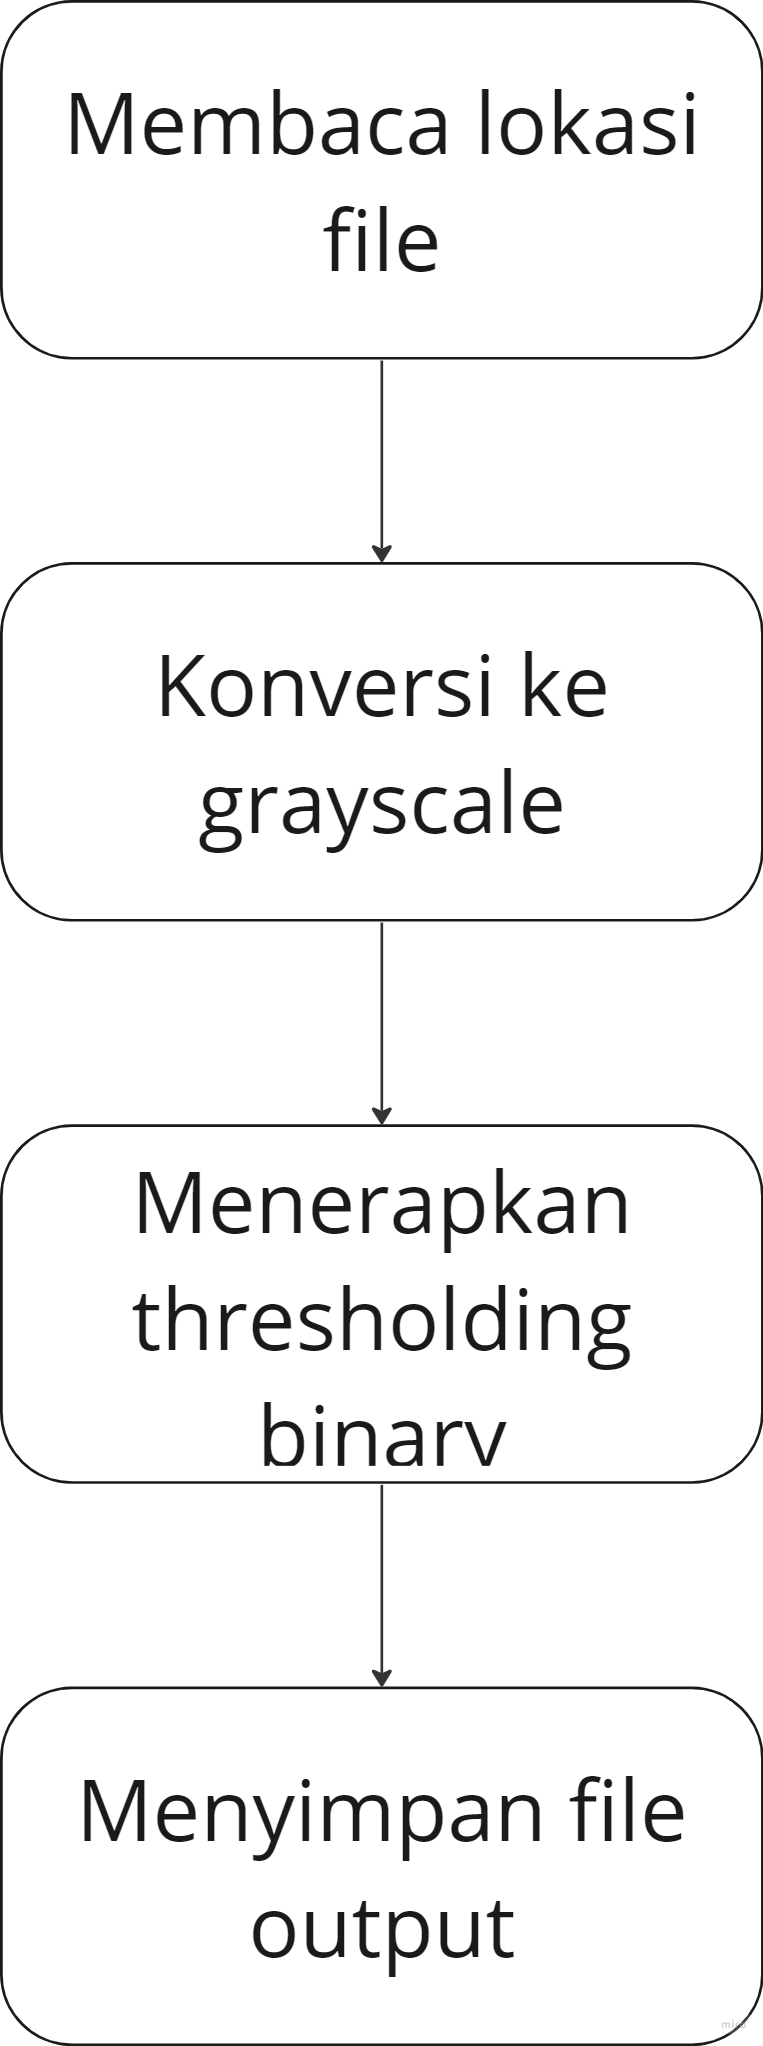
\includegraphics[scale=0.1]{gambar/bab3/preflow2.png}
  \caption{Proses Binarisasi}
  \label{fig:preflow2}
\end{figure}

\begin{algorithm}
  \caption{Process Images in a Directory}
  \begin{algorithmic}[1]
  \Function{ProcessImage}{image\_path, output\_dir}
      \State Read the image from image\_path
      \State Convert the image to grayscale
      \State Apply Otsu's thresholding to the grayscale image to obtain a binary image
      \State Construct the output path relative to output\_dir
      \State Ensure the parent directory of output path exists
      \State Save the binary image to the output path
  \EndFunction
  \State
  \Procedure{ProcessDirectory}{input\_dir, output\_dir}
      \State Convert input\_dir and output\_dir to Path objects
      \State Prepare a list of image files to process, filtering by extensions (.png, .jpg, .jpeg, .bmp)
      \For{each image\_path in the list of image files}
          \State \Call{ProcessImage}{image\_path, output\_dir}
      \EndFor
  \EndProcedure
  \State
  \State Specify the input and output directories
  \State Call \Call{ProcessDirectory}{input\_dir, output\_dir}
  \end{algorithmic}
\end{algorithm}  

Selanjutnya, flowchart diatas menjelaskan proses untuk mengubah gambar menjadi binarisasi. Pada program ini, pertama-tama dilakukan pembacaan lokasi file yang ingin diubah formatnya. Kemudian dilakukan import library yang dibutuhkan. Selanjutnya, program akan membaca gambar sinyal yang telah dihasilkan dari proses generate data. Gambar sinyal tersebut kemudian akan diubah formatnya menjadi grayscale. Setelah itu, diterapkan threshold agar gambar sinyal tersebut menjadi biner. Gambar sinyal yang telah diubah formatnya akan disimpan pada folder yang telah disediakan.

\subsection{\emph{Training} Data}
Pada proses training data menggunakan CNN 2D, perlu dilakukan penyusunan program untuk training CNN 2D pada Google Colab. Berikut ini adalah flowchart dari training data CNN 2D yang dapat dilihat pada gambar \ref{fig:trainingcnn}.

\begin{figure} [H] \centering
  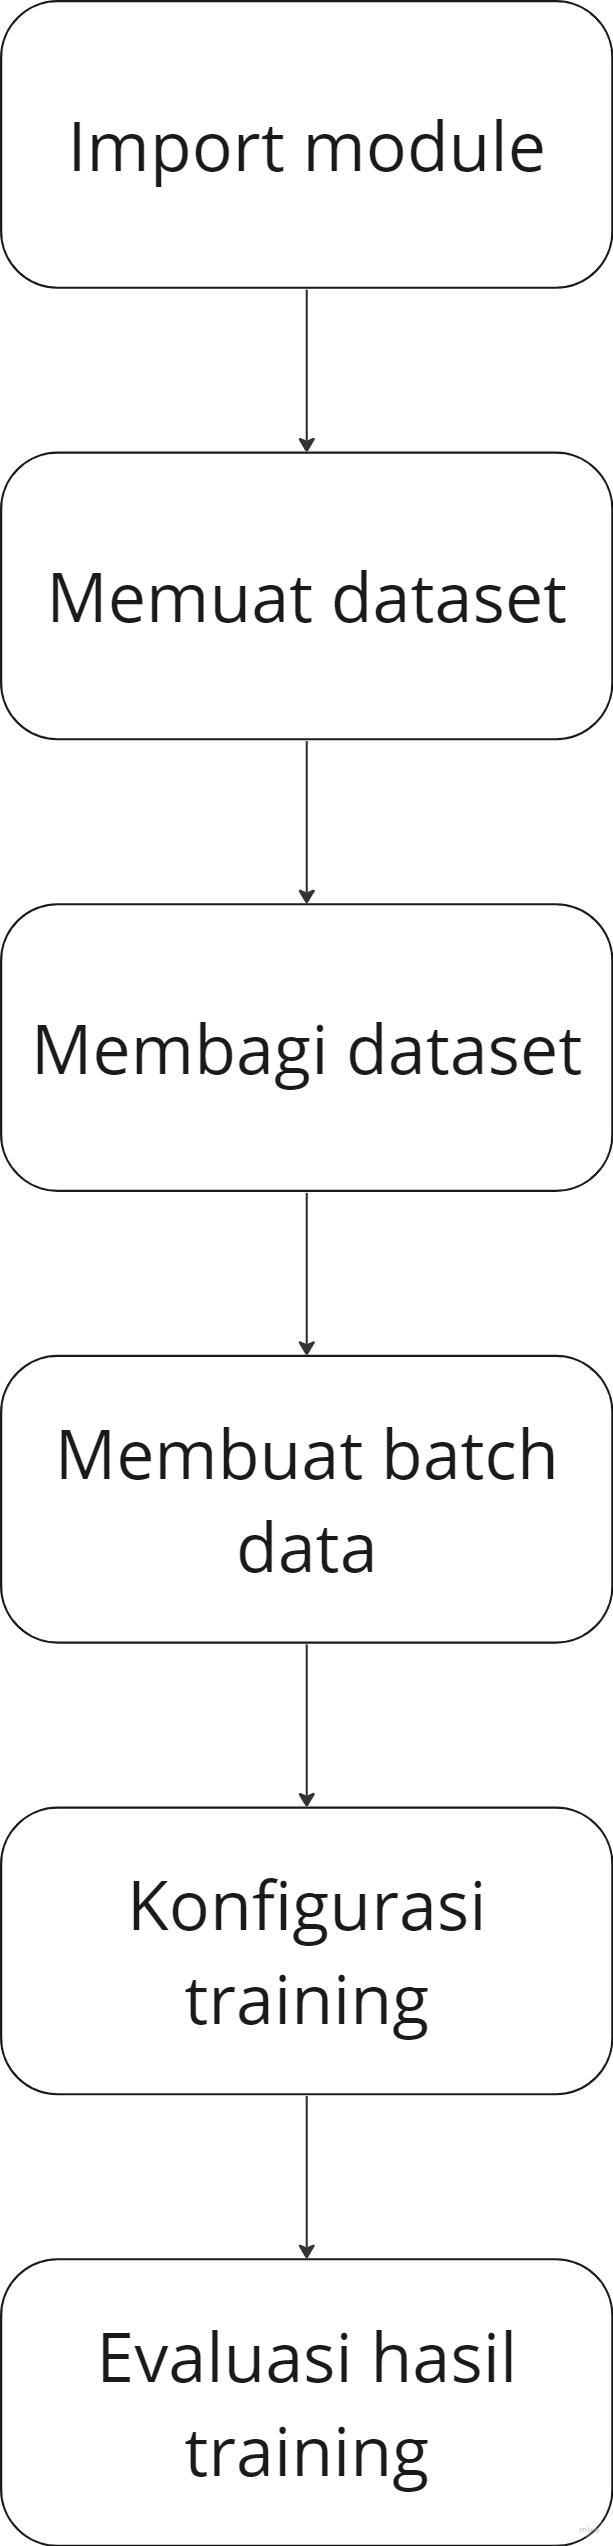
\includegraphics[scale=0.1]{gambar/bab3/trainingcnn.png}
  \caption{Training CNN 2D}
  \label{fig:trainingcnn}
\end{figure}

\begin{algorithm}
  \caption{Training and Evaluation of CNN for Image Classification}
  \begin{algorithmic}[1]
  \State Import necessary modules and libraries
  \State Mount Google Drive and set paths for datasets
  \State Initialize random seeds for reproducibility
  
  \State Define data generators with augmentation settings for training and validation
  \State Prepare data generators for training and validation subsets
  
  \Function{CreateModel}{}
      \State Define a sequential model with multiple convolutional blocks
      \State Add pooling, flattening, dense, and dropout layers
      \State Configure compilation settings (optimizer, loss, metrics)
      \State \textbf{return} model
  \EndFunction
  
  \State Instantiate the model using \Call{CreateModel}{}
  \State Print model summary
  
  \State Define EarlyStopping callback for training
  \State Train model using fit method with callbacks
  \State Evaluate model on validation and training data
  
  \State Plot accuracy and loss graphs for training and validation
  \State Save the trained model to Google Drive
  
  \State Predict on new data using test generators
  \State Display and analyze confusion matrices for training and validation sets
  
  \State Calculate and print F1 scores for training, validation, and test sets
  
  \State Annotate test images with predictions and save outputs
  
  \end{algorithmic}
\end{algorithm}

Pada CNN 2D, digunakan Google Colab sebagai platform untuk training data. Pada CNN ini, digunakan tensorflow untuk mengimport semua kebutuhan CNN 2D. Kemudian mendefinisikan dua generator data gambar, train datagen dan val datagen, yang masing-masing digunakan untuk augmentsi data training secara otomatis dan menyiapkan data validasi. Kedua generator mengubah skala nilai pixel gambar dari [0, 255] menjadi [0, 1] dengan mengalikannya dengan 1,0/255 untuk menormalisasi data. train datagen juga menerapkan transformasi acak seperti geser dan zoom (masing-masing hingga 20\%) dan mengatur fill mode ke "nearest" untuk menangani pixel di luar batas gambar selama transformasi. Generator data ini dikonfigurasi untuk membagi kumpulan data menjadi subset training dan validasi, dengan 20\% data dicadangkan untuk validasi.Kemudian gambar diproses agar sesuai dengan ukuran input model 330x540 piksel, menanganinya dalam 10 batch, dan menghasilkan gambar grayscale. Mode kelas diatur ke "biner" yang menunjukkan bahwa klasifikasi tersebut adalah klasifikasi biner.

Kode CNN ini memiliki variasi dalam layerya. Hal serupa yang dimiliki setiap variasi adalah setiap variasi dari CNN 2-Dimensi memiliki setidaknya sebuah Convolutional layer dan Dense layer yang jumlah serta pengaturan lanjutan yang berbeda-beda pada setiap eksperimen. Kemudian ditambahkan dense layer terakhir dengan unit tunggal dan aktivasi sigmoid untuk klasifikasi biner. Selanjutnya, dilakukan konfigurasi model training dengan menggunakan model.compile() yang mengatur optimizer, loss function, dan metrik evaluasi. Pada model ini, digunakan optimizer Adam dengan loss function binary crossentropy, dan metrik evaluasi akurasi. Kemudian, model dilatih dengan model.fit() yang mengatur generator data training, jumlah epoch sebanyak, generator data validasi, dan langkah validasi. Pada model ini, dilakukan training sebanyak 100 epoch dengan early stopping dan langkah validasi yang disesuaikan dengan ukuran batch dan jumlah validasi. Setelah training selesai, model disimpan dalam format .h5 dan proses training menghasilkan data yang diperlukan terkait hasil training itu sendiri.

Pada percobaan pertama, kedua, dan ketiga, digunakan model CNN 2D yang sama untuk mengetahui pembagian data yang baik. Model pada ketiga percobaan ini dapat dilihat pada tabel \ref{fig:cnnarc1} dimana model ini memiliki total 14 layer dengan rincian 4 Convolutional layer, 4 MaxPooling layer, 1 flatten layer, 2 dropout layer dan 3 dense layer. Untuk percobaaan keempat, digunakan pembagian data yang terbaik dari tiga percobaan pertama. Terdapat perbedaan pada model CNN 2D pada percobaan keempat ini dimana model ini memiliki total 18 layer dengan rincian 4 Convolutional layer, 4 MaxPooling layer, 1 flatten layer, 2 dropout layer, 3 dense layer dan 4 BatchNormalization layer yang ditambahkan setelah setiap Convolutional layer Model pada percobaan keempat ini dapat dilihat pada tabel \ref{fig:cnnarc2}. Sementara itu, pada percobaan kelima, digunakan model CNN 2D dengan layer yang lebih sedikit. Model pada percobaan kelima ini dapat dilihat pada tabel \ref{fig:cnnarc3}. Pada model tersebut, terdapat total 10 layer dengan rincian 2 Convolutional layer, 2 MaxPooling layer, 2 BatchNormalization layer, 1 flatten layer, 1 dropout layer, dan 2 dense layer. Pada percobaan keenam, digunakan model CNN 2D yang juga berbeda yang bisa dilihat pada tabel \ref{fig:cnnarc4}. Model pada percobaan keenam ini memiliki total 11 layer dengan rincian 3 Convolutional layer, 3 MaxPooling layer, 1 flatten layer, 2 dropout layer dan 2 dense layer. Pada percobaan ketujuh, digunakan model CNN 2D yang juga berbeda yang bisa dilihat pada tabel \ref{fig:cnnarc5}. Model pada percobaan keenam ini memiliki total 12 layer dengan rincian 6 Convolutional layer, 4 MaxPooling layer, 1 flatten layer dan 1 dense layer. Dari semua model yang digunakan, digunakan input size dan target size yang sama yakni 550 x 330 piksel dengan mode klasifikasi biner dan warna grayscale.

\subsection{Pengujian Klasifikasi Lanjut Revisi}
Model CNN yang telah di training, akan dilakukan pengujian klasifikasi. Klasifikasi dilaksanakan dengan menggunakan data training, validasi, dan testing. Berikut ini adalah flowchart dari pengujian klasifikasi yang dapat dilihat pada gambar \ref{fig:ujiklasifikasi}.

\begin{minipage}{\linewidth}
  \begin{figure} [H] \centering
    
\includegraphics[scale=0.1]{gambar/bab3/ujiklasifikasi.png}
    \caption{Pengujian Klasifikasi}
    \label{fig:ujiklasifikasi}
  \end{figure}
\end{minipage}

\begin{algorithm}
  \caption{Image Classification with a Pre-trained Model}
  \begin{algorithmic}[1]
  \State Mount Google Drive to access files
  \State Import necessary libraries and modules: TensorFlow, NumPy, Matplotlib
  
  \State Define class names for classification
  \State Load the pre-trained model from specified path
  
  \State Load the image from a path
  \State Preprocess the image: resize, convert color mode, normalize
  \State Expand dimensions of the image array for model input
  
  \State Perform image classification using the model
  \State Determine the predicted class based on the highest probability
  
  \State Display the image and the predicted class
  \end{algorithmic}
\end{algorithm}

Pengujian dapat dilakukan terhadap file tunggal maupun banyak file sekaligus. Pada program, dilakukan import module yang dibutuhkan dalam proses pengujian. Langkah selanjutnya, dimuat model CNN 2D yang telah di training. Kemudian, dimuat gambar yang ingin diuji klasifikasi. Setelah menjalankan proses klasifikasi, maka akan dihasilkan output berupa gambar yang telah diuji klasifikasinya dengan label kelas terklasifikasi. Untuk pengujian data secara keseluruhan, dilakukan pengujian sebagaimana yang tertera pada pseudocode subbab sebelumnya. Data yang dimuat tadi disesuaikan target ukurannya menjadi 550 x 330 piksel dengan mode klasifikasi biner dan warna grayscale. Pengaturan ini dilakukan untuk masing-masing data training, validasi, dan testing. Dilakukan prediksi pada masing-masing data tersebut yang kemudian hasilnya akan disajikan dalam bentuk confussion matrix. Confussion matrix ini akan menunjukkan hasil prediksi yang tepat dan tidak tepat dalam empat kategori yakni TP, FP, TN, dan FN. Selain itu, akan dihitung pula nilai akurasi dari model yang telah di training. Proses pengujian dilakukan lebih lanjut dengan setiap data testing yang diuji, disimpan hasil dari setiap gambar yang diuji tersebut ke dalam folder yang telah disediakan.

\subsection{Deteksi YOLOv9}
Gambar yang telah berhasil diklasifikai akan dilakukan proses deteksi menggunakan YOLOv9. Pada proses deteksi YOLO, perlu dilakukan penyusunan program untuk deteksi YOLO pada Google Colab. Berikut ini adalah flowchart dari deteksi YOLO yang dapat dilihat pada gambar \ref{fig:deteksiyolo}.

\begin{figure} [H] \centering
  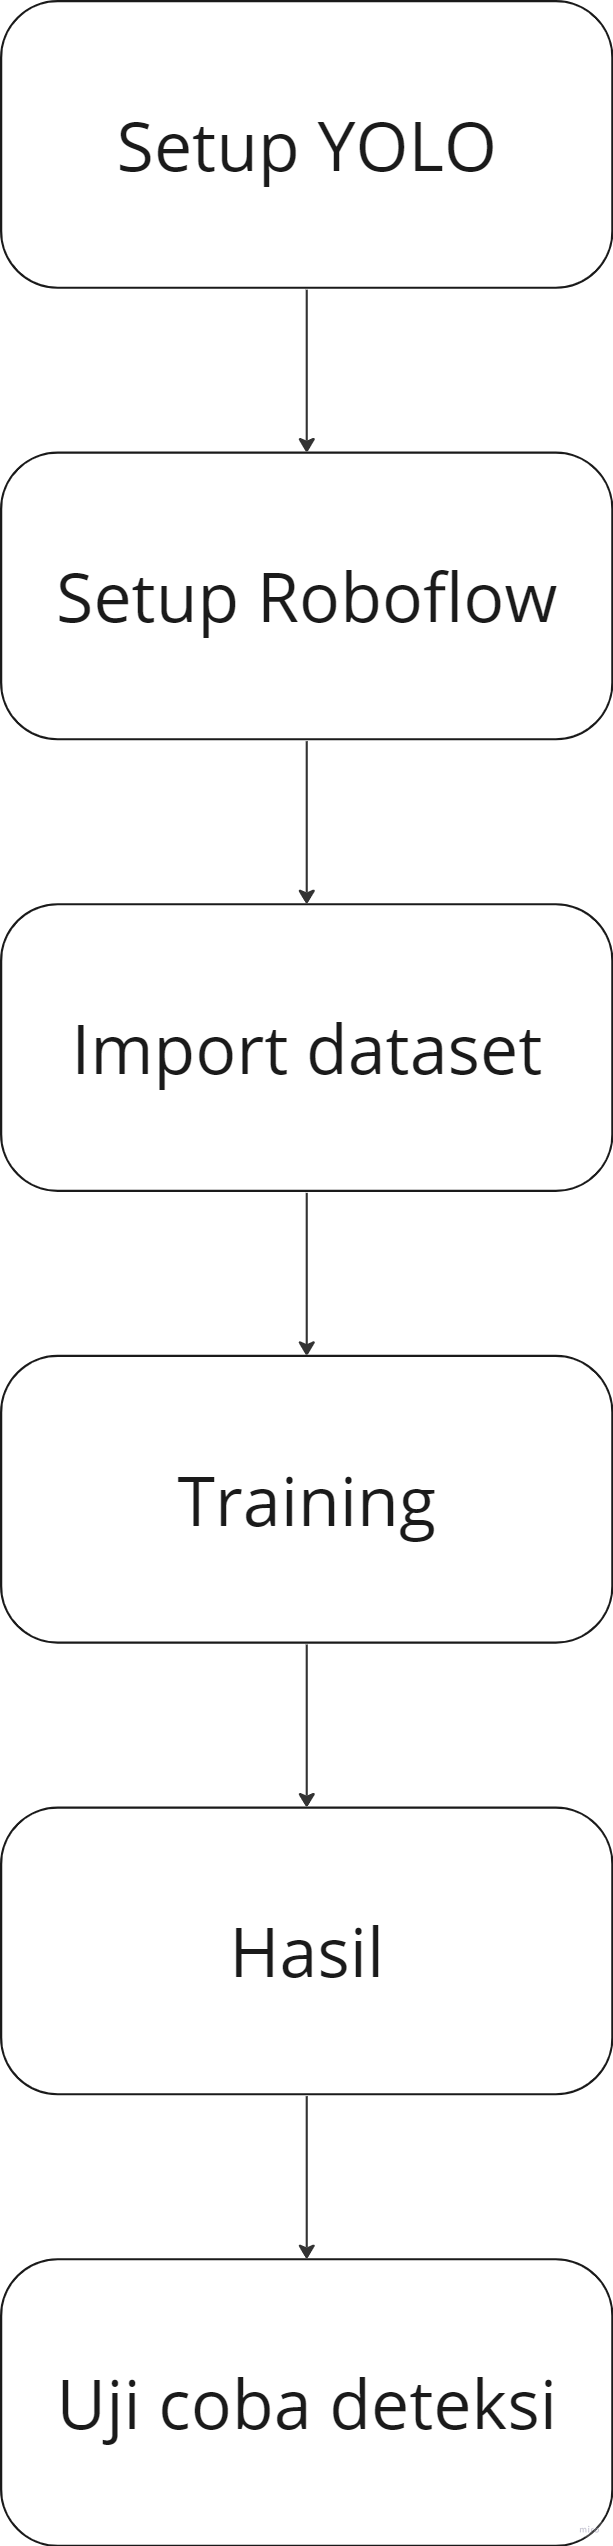
\includegraphics[scale=0.1]{gambar/bab3/deteksiyolo.png}
  \caption{Deteksi YOLOv9}
  \label{fig:deteksiyolo}
\end{figure}

\begin{algorithm}
  \caption{Training and Inference with YOLOv9 on a Custom Dataset}
  \begin{algorithmic}[1]
  \State Mount Google Drive for file access
  \State Check GPU availability using \texttt{nvidia-smi}
  \State Define the home directory and verify it with a print statement
  \State Clone YOLOv9 repository and navigate into it
  \State Install required libraries from the requirements file
  \State Install additional package, Roboflow
  
  \State Download model weights to the specified home directory weights folder
  \State Prepare the data directory within the home directory
  \State Download the dataset using Roboflow and configure it for YOLOv9
  
  \State Train the model using custom weights and hyperparameters
  \State Mount Google Drive if necessary
  \State Download the best model weights after training
  
  \State List training results including images and plots
  \State Display training result images using IPython display functionality
  
  \State Validate the custom model with specified parameters
  \State Perform detection using the trained model on validation images
  
  \State Display confusion matrix and a subset of detection result images
  \end{algorithmic}
\end{algorithm}

Pada program ini, pertama-tama dilakukan import library yang dibutuhkan. Selanjutnya, dilakukan setup YOLOv9 dengan melakukan clone YOLOv9 dari repository github yang kemudian dilakukan instalasi berdasarkan file requirement.txt agar YOLOv9 bisa bekerja. Selanjutnya, program melakukan intalasi Roboflow yang mana hal ini bertujuan agar program bisa melakukan import dari platform Roboflow karena dataset yang digunakan dianotasi pada platform tersebut. Didapatkan bobot YOLOv9 dari repository github yang telah diclone dan melakukan penyesuaian nilai jumlah kelas yang akan dideteksi sesuai dengan jumlah kelas yang ada.

Program kemudian akan melakukan import dataset dari Roboflow dimana dataset tersebut sudah dianotasi. Dilakukan proses training dengan mengatur beberapa parameter seperti ukuran batch, jumlah epoch, ukuran gambar. Ukuran batch diatur menjadi 8, jumlah epoch diatur menjadi 10, dan ukuran gambar diatur menjadi 640x640 piksel menyesuaikan dengan dataset yang telah dilakukan bounding box pada Roboflow. Setelah proses training, didapatkan nilai dari akurasi model tersebut. Kemudian dilakukan prediksi pada yang telah tersedia.